\documentclass[12pt]{article}

\usepackage[utf8]{inputenc}
\usepackage[margin = 1in]{geometry}
\usepackage[english]{babel}
\usepackage{amsthm}
\usepackage{amssymb}
\usepackage{amsmath}
\usepackage{changepage}
\usepackage[makeindex]{imakeidx}
\usepackage{titlesec}
\usepackage{textcomp}
\usepackage{graphicx}
\usepackage{gensymb}
\usepackage{xcolor, soul}
\usepackage{hyperref}
\usepackage{pgfplots}
\usepackage{parskip}

\graphicspath{ {./images/} }

\definecolor{linkColour}{RGB}{140, 25, 57}
\definecolor{urlColour}{RGB}{137, 62, 27}

\setcounter{section}{-1}
\setcounter{secnumdepth}{4}

\titleformat{\paragraph}
{\normalfont\normalsize\bfseries}{\theparagraph}{1em}{}
\titlespacing*{\paragraph}
{0pt}{3.25ex plus 1ex minus .2ex}{1.5ex plus .2ex}

\hypersetup{colorlinks, citecolor=purple, filecolor=purple, linkcolor=linkColour, urlcolor=urlColour}

\makeindex

\newcommand{\homl}{\hyperlink{homl}{Hands-On Machine Learning}}

\newenvironment{fact*}[2][]
    {
    \begin{adjustwidth}{1em}{0em}
    \noindent
    \textbf{#2} \hfill #1
    
    \vspace{0.1in}
    \noindent
    \ignorespaces
    } {
    \end{adjustwidth}
    }

\newenvironment{fact}[2][]
    {
    \index{#2}
    \hypertarget{#2}{\vspace{0.2in}}
    \begin{adjustwidth}{1em}{0em}
    \noindent
    \textbf{#2} \hfill #1
    
    \vspace{0.1in}
    \noindent
    \ignorespaces
    } {
    \end{adjustwidth}
    }

\title{Companion to Machine Learning}
\author{Rohan Kumar}
\date{}






\begin{document}

\maketitle
\newpage
\tableofcontents
\newpage

\section*{Sources}
    Throughout this compendium, each piece of information will be formatted as such.
    
    \vspace{0.1in}
    \begin{fact*}[Source]{Name / Description of fact}
        Information about fact.
    \end{fact*}
    \vspace{0.3in}
    
    \noindent The location which currently contains ``Source'' could potentially be filled with a variety of sources.
    Here is how to find the source based off the shortened form.
    
    \begin{itemize}
        \item \hypertarget{homl}{\textbf{Hands-On Machine Learning}} refers to Hands-On Machine Learning with
        Scikit-Learn, Keras, and TensorFlow, 2nd Edition by Aurélien Géron
    \end{itemize}

\newpage

\section{Notation}
    \subsection{Data}
    \begin{flalign*}
        \boldsymbol{x} &= \begin{pmatrix} x_1 \\ x_2 \\ ... \\ x_M \end{pmatrix} \text{: data point corresponding to a
        column vector of $M$ features} & \\
        \overline{\boldsymbol{x}} &= \begin{pmatrix} 1 \\ x_1 \\ x_2 \\ ... \\ x_M \end{pmatrix} \text{: concatenation
        of 1 with the vector} \boldsymbol{x} & \\
        \boldsymbol{X} &= \begin{pmatrix} x_{1,1} & ... & x_{1,N} \\ ... & ... & ... \\ x_{M,1} & ... & x_{M,N}
        \end{pmatrix} \text{: dataset consisting of $N$ data points and $M$ features} & \\
        \overline{\boldsymbol{X}} &= \begin{pmatrix} 1 & ... & 1 \\ x_{1,1} & ... & x_{1,N} \\ ... & ... & ... \\
        x_{M,1} & ... & x_{M,N} \end{pmatrix} \text{: concatenation of a vector of 1's with the matrix } \boldsymbol{X}
        & \\
        y &= \text{: output target (regression) or label (classification)} & \\
        \boldsymbol{y} &= \begin{pmatrix} y_1 \\ y_2 \\ ... \\ y_N \end{pmatrix} \text{: vector of outputs for a dataset
        of $N$ points} & \\
        \boldsymbol{x}_* &= \text{: test input / unknown input } & \\
        \boldsymbol{y}_* &= \text{: predicted output} & \\
        N &= \text{: Number of data points in the dataset} & \\
        M &= \text{: Number of a features in a data point} & \\
        \boldsymbol{w} &= \begin{pmatrix} w_1 \\
            w_2 \\
            ... \\
            w_M \\
        \end{pmatrix} & \\
        \boldsymbol{w}^T &= (w_1, w_2, ..., w_M) \text{ or } (w_0, w_1, w_2, ..., w_M) \text{ $w_0$ multiplies the first
        entry of $\overline{\boldsymbol{x}}$ (bias)} & \\
    \end{flalign*}
    Note: bold symbols represents a vector

\section{Introduction}

\subsection{What is Machine Learning}
    Machine Learning is the field of study that gives computers the ability to learn from data without being explicitly
    programmed. This is good for problems that require a lot of fine-tuning or for which using a traditional approach
    yields no good solution. Machine Learning's data dependency allows it to adapt to new data and gain insight for
    complex problems and large amounts of data.

\subsection{Applications of Machine Learning}
    Machine Learning can be used for a range of tasks and can be seen used in:
    \begin{itemize}
        \item Analyzing images of products on a production line to automatically classify them (Convolutional Neural
        Net)
        \item Forecasting company revenue based on performance metrics (Regression or Neural Net)
        \item Automatically classifying news articles (NLP using Recurrent Neural Networks)
        \item Summarizing long documents automatically (Natural Language Processing)
        \item Building intelligent bot for a game (Reinforcement Learning)
    \end{itemize}

\subsection{Types of Machine Learning}
    \subsubsection{Supervised Learning}
        In supervised learning, the training set you feed to the algorithm includes the desired solutions, called
        labels. (e.g determining if an email is spam would be trained a dataset of example emails labelled as spam or
        not spam.) \\[0.1in] 
        Some commonly used supervised learning algorithms are:
        \begin{itemize}
            \item \hyperref[sec:KNN]{k-Nearest Neighbors}
            \item \hyperref[sec:LinearRegression]{Linear Regression}
            \item \hyperref[sec:LogisticRegression]{Logistic Regression}
            \item Support Vector Machines (SVMs)
            \item Decision Trees and Random Forests
            \item Neural Networks
        \end{itemize}
    
    \subsubsection{Unsupervised Learning}
        In unsupervised learning, the training data is unlabeled and the system tries to learn without guidance. The
        system will try and automatically draw inferences and conclusions about the data and group it as such. (e.g.
        having a lot of data about blog visitors. Using a clustering algorithm we can group and detect similar
        visitors). \\[0.1in]
        Some important unsupervised learning algorithms are:
        \begin{itemize}
            \item Clustering
            \begin{itemize}
                \item K-Means
                \item DBSCAN
                \item Hierarchical Cluster Analysis
            \end{itemize}
            \item Anomaly detection and novelty detection
            \begin{itemize}
                \item One-class SVM
                \item Isolation Forest
            \end{itemize}
            \item Visualization and dimensionality reduction
            \begin{itemize}
                \item Principal Component Analysis (PCA)
                \item Kernel PCA
                \item Locally Linear Embedding (LLE)
                \item t-Distributed Stochastic Neighbor Embedding (t-SNE)
            \end{itemize}
            \item Association rule learning
            \begin{itemize}
                \item Apriori
                \item Eclat
            \end{itemize}
        \end{itemize}

    \subsubsection{Semisupervised Learning}
        Labelling can be very time-consuming and costly, often there will be plenty of unlabelled and a few labelled
        instances. Algorithms that deal with data that is partially labeled is called semi-supervised learning. A good
        example of this is Google Photos. Google clusters and groups your photos based on facial recognition
        (unsupervised) and then you can label one photo and it will be able to label every picture like that
        (supervised). Most semi-supervised learning algorithms are combinations of unsupervised and supervised
        algorithms.  
    
    \subsubsection{Reinforcement Learning}
        Reinforcement Learning is a learning algorithm based on a reward system. The learning system, called an agent,
        can observe the environment, select and perform actions, and get rewards in return (or penalties in the form of
        negative rewards). It will then learn by itself what the best strategy, called a policy, to get the most reward
        over time. A policy defines what action the agent should choose when it is in a given situation.

\section{Data Analysis}
    \subsection{Limitations of Data}
        \subsubsection{Nonrepresentative Training Data}
        One thing to look out for when using training data is whether the data is representative of the new cases you
        want to generalize to. For example if you are training linear regression life satisfaction vs GDP of countries,
        if some countries are missing from the dataset then the dataset is not fully representative of the problem.

        \subsubsection{Poor Quality Data}
        If your data is full of errors, outliers and noise, it will make it harder for the system to detect the
        underlying patterns, so your system is less likely to perform well. In order to mitigate this we need to clean
        the training data.
        \begin{itemize}
            \item If some instances are outliers, it may help to discard them or try to fix the errors manually
            \item If some instances are missing features, you may decide to ignore that attribute, ignore the instance,
            fill in the missing values, or train one model with the feature and one without
        \end{itemize}

        \subsubsection{Irrelevant Features}
        A critical part of the success of a Machine Learning project is coming up with a good set of features to train
        on. This process is called \hyperref[sec:FeatureEngineering]{\textit{feature engineering}}.
        \begin{itemize}
            \item \hyperref[sec:FeatureSelection]{\textit{Feature selection}}: Selecting the most useful features to
            train on among the existing features
            \item \hyperref[sec:FeatureExtraction]{\textit{Feature extraction}}: Combining existing features to produce
            a more useful one (dimensionality reduction algorithms can help)
            \item \hyperref[sec:AdhocFeatures]{\textit{Ad hoc Features}}: Creating new features by gathering new data.
        \end{itemize}

    \subsection{Feature Engineering} \label{sec:FeatureEngineering}
        \subsubsection{Feature Construction}
            Features can be modified for various reasons, including to increase predictor performance and to reduce time
            or memory requirements. Below are common techniques for constructing features.

            \paragraph{Transformation}
            Common feature transformations include:
            \begin{itemize}
                \item \textbf{Centering} each feature to be around the origin.
                \item \textbf{Scaling} each feature to be of the same scale. For example, scaling can be done to make
                sure each feature has the same variance or the same maximum absolute value.
                \item \textbf{Logarithmically} transforming each feature to reduce the skewness of feature
                distributions.
            \end{itemize}

            Note that feature transformation runs the risk of discarding useful information. For example, scaling to
            make each feature have the same variance should not be done if the differing variances of the features are
            actually relevant to the problem.

            \paragraph{Feature Extraction} \label{sec:FeatureExtraction} Feature expansion involves combining multiple
            features into new features when first order interactions are not good enough. For example, given features
            $x_1$ and $x_2$, $x_1 \cdot x_2$ is a new feature (i.e. meta-feature) formed by an expansion of $x_1$ and
            $x_2$.

            \paragraph{``Ad hoc'' Features} \label{sec:AdhocFeatures} Constructing ad hoc features involves applying
            domain knowledge to introduce custom features.

        \subsubsection{Feature Selection} \label{sec:FeatureSelection} Irrelevant features are features that are
            uncorrelated with a prediction task. Redundant features are features that are highly correlated with one
            another, so using multiple redundant features does not help with predictions much more than using a single
            such feature.

            Different learning algorithms have differing levels of robustness to irrelevant or redundant features. For
            example, decision trees are robust to redundant features, since such features have low information gain,
            while KNN is not, since the set of redundant features will behave as one heavily weighted feature. When
            possible, these feature should not be selected in the first place. Below are common ways to avoid selecting
            such features.

            \paragraph{Wrapper Methods}
            Wrapper methods involve building a model for feature subsets, and then selecting the best performing model.
            A ``forward search'' approach starts with no features and then adds the feature that best improves the model
            until a certain number of features are selected.  A ``backward'' search approach starts with all features
            and removes the feature that improves the model the least until a certain number of features have been
            removed.

            Computing all possible feature subsets would guarantee finding the optimal one. However, a problem with $M$
            features has $2^M$ possible feature subsets, so finding all possible subsets is infeasible for large values
            of $M$. The forward and backward search approaches approximate this but with a time complexity of $O(M^2)$.

            \paragraph{Filter Methods}
            Filter methods, also known as variable ranking, involve assigning each feature a score measuring how
            informative it is in predictions. This score is determined by some ``scoring function'' $S$. Features are
            then ranked by score, and a number of top features are selected.

            \paragraph{Embedded Methods}
            Embedded methods involve  modifying the cost function to constrain the choice of model. A common example of
            this is regularization, which can be used to penalize complex models and encourage a sparse feature set.

    \subsection{Overfitting} \label{sec:Overfitting}
        \textit{Overfitting} is when the model performs well on the training data, but does not generalize well. Complex
        models can detect subtle patterns in the data, but if the training set is noise, or if it is too small, then the
        model will likely detect patterns in the noise itself. These patterns will not generalize to new instances.
        Overfitting often happens when the training data has many features, which allows for an approximation of the
        target function with many degrees of freedom. We can use regularization to constrain a model to make it simpler
        to reduce the risk of overfitting.

    \subsection{Underfitting} \label{sec:Underfitting}
        \textit{Underfitting} is the opposite of overfitting: it occurs when the model is too simple to learn the
        underlying structure of the data. Methods of fixing the problem include:
        \begin{itemize}
            \item Select a more powerful model, with more parameters.
            \item Feed better features to the learning algorithm
            \item Reduce the constraints on the model (e.g., reduce the regularization hyperparameter)
        \end{itemize}

    \subsection{Bias Variance Decomposition}
        Many machine learning algorithms are based on building a formal model based on the training data (e.g. a
        decision tree). Models have parameters, which are characteristics that can help in classification (e.g. a node
        in a decision tree). Models may also have hyper-parameters, which in turn control other parameters in a model
        (e.g. max height of decision tree).

        Generalization errors result from a combination of noise, variance, and bias. Bias concerns how well the type of
        model fits the data. Models with high bias pay little attention to training data and suffer from underfitting,
        while models with low bias may pay too much attention to training data and become overfitted. Bias and variance
        tend to be at odds with one another (high bias typically leads to low variance, and vice versa).

\section{Evaluation of Learning}
    \subsection{Performance Formulation}
        Let $y_*$ be an output generated by a function $f$ approximating some target function. Let $y$ be the
        corresponding output of the target function. A loss function \label{fact:LossFunction} $l(y, y_*)$ can be used
        to measure the accuracy of the approximation function $f$. Some common loss functions include:
        \begin{itemize}
            \item Squared Loss: $l(y, y_*) = (y - y_*)^2$
            \item Absolute Loss: $l(y, y_*) = |y - y_*|$
            \item Zero/One Loss: $l(y, y_*) = 1_{y \neq y_*}$
        \end{itemize}

        We assume that the data coming from our target function comes from some probability distribution $D$, and that
        our training data is a random sample of $(x, y)$ pairs from $D$. A Bayes Optimal Classifier is a classifier that
        for any input $x$, returns the $y$ most likely to be generated by $D$.

        Based on the available training data, the goal of supervised learning is to find a mapping $f$ from $x$ to $y$
        such that generalization error $\sum_{(x,y)} D(x,y)l(y,f(x))$ is minimized. However, since $D$ is unknown, we
        instead estimate the error from the average error in our training or test data, which is
        $\frac{1}{N}\sum_{n=1}^N l(y_n, f(x_n))$.

    \subsection{Testing and Validation}
        Models are initially built based on a training dataset. Test sets (also known as holdout sets) are then used to
        estimate the generalization error. Validation sets are also used to measure the model's performance, but unlike
        test sets, validation sets can make changes to the model's parameters.

        \subsubsection{Cross Validation}
            Cross validation is a technique for measuring how well a model generalizes. The idea behind it is to break
            up a training data set into $K$ equally sized partitions, and use $K-1$ of the partitions as training data
            and the remaining partition for testing. This should be repeated $K$ times, so that all points of data are
            at some point used for testing. Higher values of $K$ lower the amount of variance of in the error
            estimation. To avoid training and testing data having a different probability distribution, the data should
            be shuffled before being split.

        \subsubsection{Bootstrapping}
            Bootstrapping is an alternative to cross validation where instead of dividing a training data set into
            partitions, a random sample of points (with possible duplicates) is used as training data. The remaining
            points are then used as testing data, with the goal being similar to that of cross validation.
    
    \subsection{Performance Evaluation of Classifiers}
        Consider the following terminology for classification problems:
        \begin{itemize}
            \item True positive ($TP$) - Examples of class 1 predicted as class 1
            \item False positive ($FP$) - Examples of class 0 predicted as class 1 (Type 1 Error)
            \item True negative ($TN$) - Examples of class 0 predicted as class 0
            \item False negative ($FN$) - Examples of class 1 predicted as class 0 (Type 2 Error)
        \end{itemize}
    
        \subsubsection{Accuracy and Error}
            The following formulas can be used to measure accuracy and error:
            $$Accuracy = \frac{TP + TN}{TP + TN + FP + FN}$$
            $$ErrorRate = \frac{FP + FN}{TP + TN + FP + FN}$$
    
        \subsubsection{Precision and Recall}
            Precision and recall can be measured as follows:
            $$P = \frac{TP}{TP + FP}$$
            $$R = \frac{TP}{TP + FN}$$
    
            Precision measures the ratio of positive predictions that were correct, while recall measures the ratio of
            total positive instances that were predicted. Similarly to how variance and bias are often at odds with one
            another, so are precision and recall.
    
        \subsubsection{F-Measure}
            An F-measure (also known as a F1 score) measures a model's accuracy by taking into account both precision
            and recall as follows:
            $$F = \frac{2PR}{P + R}$$
    
            To adjust the relative importance of precision vs recall, a weighted F-measure can be used, which is defined
            as follows:
            $$F = \frac{(1 + \beta^2)PR}{\beta^2 P + R}$$
    
            In a standard F-measure, $\beta = 1$, $\beta < 1$ means that precision is valued over recall, while $\beta >
            1$ means recall is valued over precision.
    
        \subsubsection{Sensitivity and Specificity}
            Sensitivity is the same measure as recall. Specificity is a measure of how well a classifier avoids false
            positives, and is measured as:
            $$Specificity = \frac{TN}{TN + FP}$$

\section{Activation Functions} \label{sec:ActivationFunction}
    \subsection{Linear/Identity} \label{sec:Identity}
        The \textit{linear function} is an activation function where the output is proportional to the input and the
        \textit{identity function} is a subset of the linear function where $a = 1$. 
        $$ h(x) = ax $$

        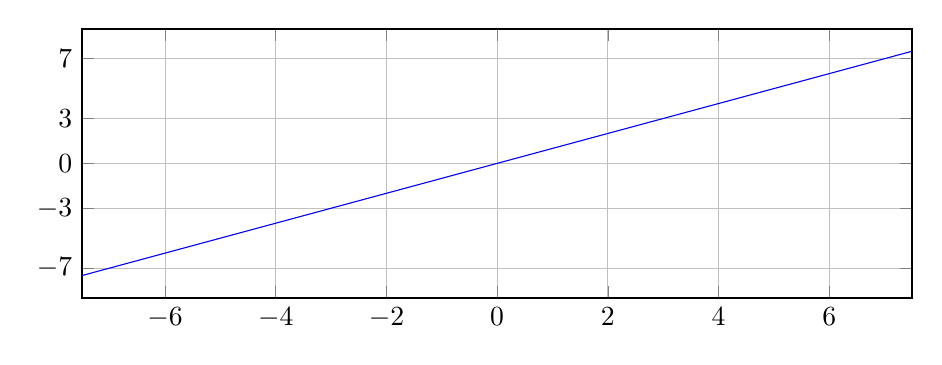
\begin{tikzpicture}
            \begin{axis}
            [%
                axis line style = thick, grid=major, xmin=-7.5, xmax=7.5, ytick={-7,-3,0,3,7}, width = \linewidth, height =
                5cm] \addplot%
                [
                    blue,%
                    mark=none,
                    samples=100,
                    domain=-7.5:7.5,
                ]
                {x};
            \end{axis}
        \end{tikzpicture}

        The linear function gives a range of activations so it is not a binary activation. The derivative is
        constant so the gradient has no relationship with $\boldsymbol{X}$ and therefore backpropagation and gradient
        descent would not work with this activation function.

    \subsection{Threshold} \label{sec:Threshold}
        The \textit{threshold function} denoted $heaviside(\cdot)$ outputs a number 0 or 1 based on its input $z$. It is defined as a piecewise function
        \[
            heaviside(z) = 
            \begin{cases}
                0 & \text{if $z < 0$} \\
                1 & \text{if $z \geq 0$}
            \end{cases}
        \]

        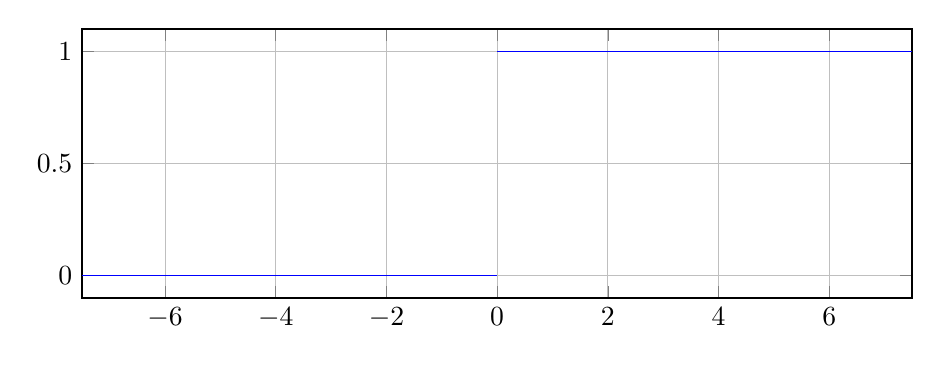
\begin{tikzpicture}
            \begin{axis}
            [%
                axis line style = thick, grid=major, xmin=-7.5, xmax=7.5, ytick={0,.5,1}, width = \linewidth, height =
                5cm]
                \addplot%
                [
                    blue,%
                    mark=none,
                    samples=100,
                    domain=-7.5:0,
                ]
                {0};

                \addplot%
                [
                    blue,%
                    mark=none,
                    samples=100,
                    domain=0:7.5,
                ]
                {1};
            \end{axis}
        \end{tikzpicture}

        The key property of the threshold function is that it will predict $1$ when $z$, which will generally be our
        prediction $\boldsymbol{w}^T\boldsymbol{x}$, is greater than $0$ else it will predict $0$.

    \subsection{Sigmoid Function} \label{sec:Sigmoid}
        The \textit{sigmoid function} denoted $\sigma(\cdot)$ outputs a number between 0 and 1. It is defined as
        $$ \sigma(t) = \frac{1}{1 + exp(-t)} $$

        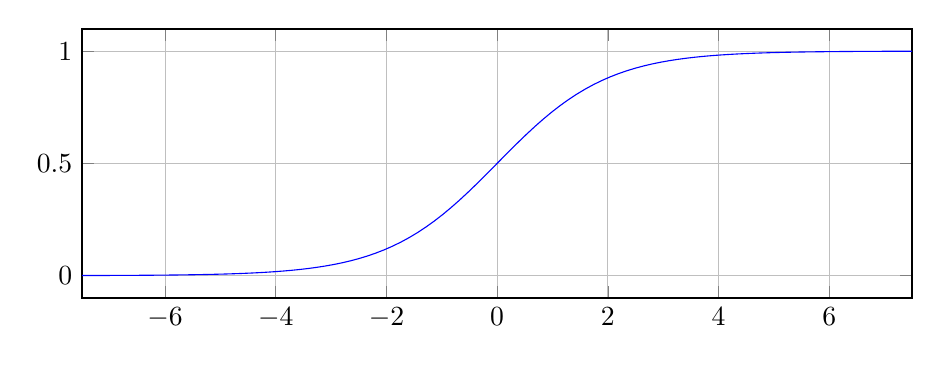
\begin{tikzpicture}
            \begin{axis}
            [%
                axis line style = thick, grid=major, xmin=-7.5, xmax=7.5, ytick={0,.5,1}, width = \linewidth, height =
                5cm] \addplot%
                [
                    blue,%
                    mark=none,
                    samples=100,
                    domain=-7.5:7.5,
                ]
                (x,{1/(1+exp(-x))});
            \end{axis}
        \end{tikzpicture}

        The key property of the sigmoid function is that $\sigma(t) < 0.5$ when $t < 0$, and $\sigma(t) \geq 0.5$ when
        $t \geq 0$, so a sigmoid function is useful for classification since it can predict 1 when
        $\boldsymbol{w}^T\boldsymbol{x}$ is positive and 0 if it is negative.

    \subsection{Tanh} \label{sec:Tanh}
        The \textit{tanh function} denoted $tanh(\cdot)$ outputs a number between -1 and 1. It is zero-centered function making it easier to
        model inputs that have strongly negative, neutral, and strongly positive values, otherwise it is similar to the \hyperref[sec:Sigmoid]{sigmoid
        function}.
        $$ h(a) = tanh(a) = \frac{e^a - e^{-a}}{e^a + e^{-a}} $$

        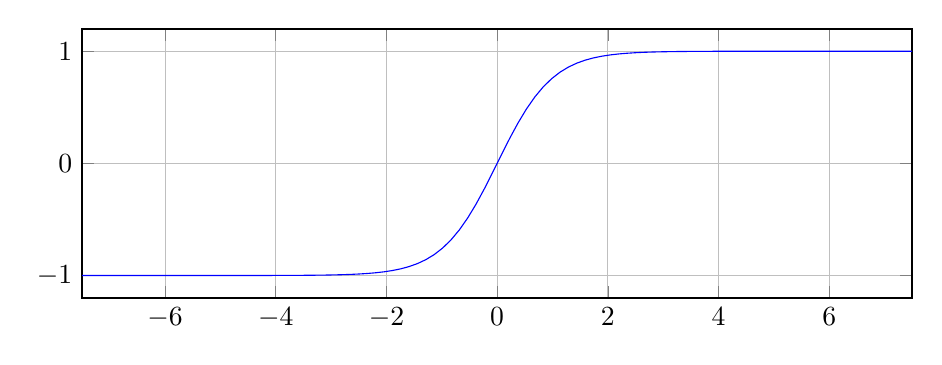
\begin{tikzpicture}
            \begin{axis}
            [%
                axis line style = thick, grid=major, xmin=-7.5, xmax=7.5, ytick={-1,0,1}, width = \linewidth, height =
                5cm] \addplot%
                [
                    blue,%
                    mark=none,
                    samples=100,
                    domain=-7.5:7.5,
                ]
                {(e^x - e^(-x))/(e^x + e^(-x))};
            \end{axis}
        \end{tikzpicture}

        The gradient is stronger for tanh than sigmoid, however, tanh also has the
        \hyperref[sec:VanishingProblem]{vanishing gradient problem}.

    \subsection{Rectified Linear Units} \label{sec:reLU}
        The \textit{reLU function} plotted in blue is defined as
        $$ h(a) = max(0, a) $$

        and the soft version ("Softplus") plotted in red is defined as
        $$ h(a) = log(1 + e^a) $$

        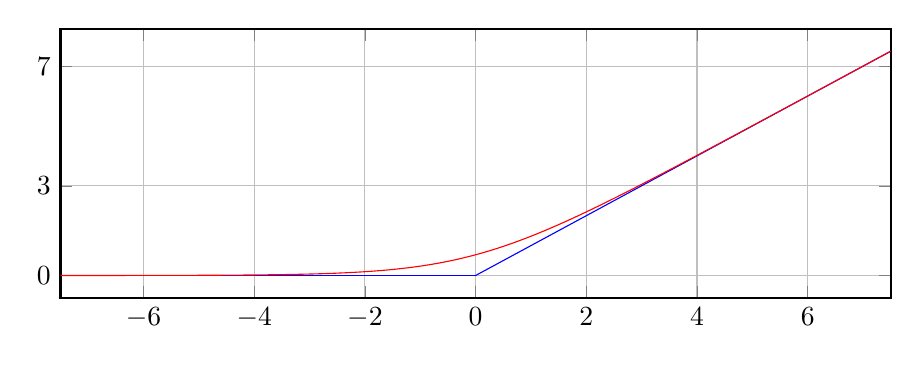
\begin{tikzpicture}
            \begin{axis}
            [%
                axis line style = thick, grid=major, xmin=-7.5, xmax=7.5, ytick={0,3,7,10}, width = \linewidth, height =
                5cm]
                \addplot%
                [
                    blue,%
                    mark=none,
                    samples=100,
                    domain=-7.5:0,
                ]
                {0};

                \addplot%
                [
                    blue,%
                    mark=none,
                    samples=100,
                    domain=0:7.5,
                ]
                {x};

                \addplot%
                [
                    red,%
                    mark=none,
                    samples=100,
                    domain=-7.5:7.5,
                ]
                {ln(1+e^x)};
            \end{axis}
        \end{tikzpicture}
        
        The benefit of using the reLU activation function is that the gradient is 0 or 1 so it helps mitigate the
        \hyperref[sec:VanishingProblem]{vanishing problem} for deep neural networks. The softplus function does not
        prevent gradient vanishing.
        
        \subsubsection{Maxout Units} \label{sec:MaxoutUnits}
            Generalization of rectified linear units where we can have several linear parts and having
            them be whatever we want rather than having a $0$ part. They can be thought of as the aggregation of a hidden
            layer of identity units with a max unit.

            $$ max \{ \sum_i w_i^{(1) x_i, \sum_i w_i^{(2)}} x_i, \sum_i w_i^{(3)}x_i, ...\} $$

\section{Convex Optimization} \label{sec:ConvexOptimization}
    In machine learning we can often turn problems into convex functions and simplify the problem into finding the
    global minima of the function, which in essence is minimizing the training error. One of the key theorem's of a
    convex function is that the local minimum of a convex function is also a global minimum. Therefore we can apply many
    methods to find parameters that satisfy the global minima.

    \subsection{Normal Solution} \label{sec:NormalSolution}
        To find the value of our parameter (generally $\boldsymbol{w}$) that minimizes the cost function, there is a
        closed-form solution. We can express this closed form solution for any convex loss function as follows.
        $$ \frac{\partial J(\boldsymbol{w})}{\partial \boldsymbol{w}} = 0 $$
        
        The limitations of using the Normal Solution is that we usually have to compute the inverse of
        $\boldsymbol{X}^T\boldsymbol{X}$ which is a $(M+1) \times (M+1)$ matrix (where $M$ is the number of features).
        The computational complexity of inverting such a matrix is typically about $O(M^{2.4})$ to $O(M^{3})$, depending
        on the implementation. Some of the other approaches below are better suited for cases where there are a large
        number of features or too many training instances to fit in memory.

    \subsection{Gradient Descent} \label{sec:GD}
        Gradient Descent is a generic optimization algorithm capable of finding optimal solution to a wide range of
        problems. The general ida is to tweak parameters iteratively in order to minimize a cost function. The main
        concept utilized in gradient descent is to measure the local gradient of the error with regard to the parameter
        vector and move in the direction of the descending gradient. Once the gradient is zero, you have reached the
        minimum.

        You start with filling your parameter $\boldsymbol{w}$ with random values (random initialization. Then you
        improve it gradually, taking small steps at a time, each step attempting to decrease the cost function, until
        the algorithm converges to a minimum. One important parameter of Gradient Descent is the size of the steps,
        determined by the \textit{learning rate} hyperparameter. If the learning rate is too small, then the algorithm
        will have to go through many iterations to converge, if the learning rate is too high, you might jump across the
        minimum possibly, higher than you were before and potentially make the algorithm diverge. One gradient descent
        technique is having a learning rate that changes as you approach the minimum to prevent overshoot, also called
        the learning schedule.

        A limitation of Gradient Descent is when the cost function we are dealing with is not a convex function. In this
        case holes, ridges, irregular terrain will make the convergence to the minimum difficult.

        \subsubsection{Batch Gradient Descent}
            To implement Gradient Descent, you need to compute the gradient of the cost function with regard to each
            model parameter $w_j$ - how much the cost function will change if you change $w_j$ a little bit. This is
            equivalent to the partial derivative of the cost function with regard to the parameter $w_j$. For the entire
            parameter vector $\boldsymbol{w}$ we can denoted the gradient vector as $\nabla_{\boldsymbol{w}}
            J(\boldsymbol{w})$.

            Once we have the gradient vector, which points uphill, we descend in the opposite direction (subtract
            $\nabla_{\boldsymbol{w}} J(\boldsymbol{w})$ from $\boldsymbol{w}$). This is where we use our learning rate
            $\alpha$ to determine the size of the downhill step.
            $$ \boldsymbol{w}^{(next step)} = \boldsymbol{w} - \alpha \nabla_{\boldsymbol{w}} J(\boldsymbol{w}) $$

            The limitation of Batch Gradient Descent is the fact that it uses the whole training set to compute the
            gradients at every step, which makes it very slow when the training set is large.
        
        \subsubsection{Stochastic Gradient Descent}
            Stochastic Gradient Descent picks a random instance in the training set at every step and computes the
            gradients based on only that single instance. This makes the algorithm much faster and also makes it
            possible to train on huge training sets. However, due to its stochastic nature, this algorithm will bounce
            up and down, decreasing only on average. Over time it will end up very close to the minimum, but once it
            gets there it will continue to bounce around, never settling down. Therefore, once the algorithm stops, the
            final parameter values are good, but not optimal.

            This can actually help when the cost function is very irregular (not convex) as it can help the algorithm
            jump out of a local minima. One solution to the problem of being unable to settle at the minimum is
            gradually reducing the learning rate. The steps start out large (helps make quick progress and escape local
            minima), then get smaller and smaller, allowing the algorithm to settle at the global minima. The function
            that determines the learning rate is called the \textit{learning schedule}.
        
        \subsubsection{Mini-batch Gradient Descent}
            Mini-batch GD is a combination of Batch GD and Stochastic GD. At each step, instead of computing the
            gradients based on the full training set or based on just one instance, Mini-batch GD computes the gradient
            on small random sets of instances called \textit{mini-batches}. The main advantage of this over Stochastic
            GD is that you get a performance boost from hardware optimization of matrix operations. Mini-batch will
            perform better to get closer to the minimum than Stochastic GD but it may be harder for it to escape local
            minima.
    
    \subsection{Gradient Descent Optimization} \label{sec:GDO}
        When training neural networks there can be issues involving slow convergence, dimensionality and magnitude. So
        other methods were introduced to be able to quickly train neural networks with accuracy for large amounts of
        data.
        
        \subsubsection{Adaptive Gradients} \label{sec:AdaGrad}
            Adagrad is an algorithm for gradient-based optimization that adapts to the learning rate to the parameters,
            performing smaller updates for parameters associated with frequently occurring features and larger updates for
            parameters associated with infrequent features. It is well suited for dealing with sparse features.

            $$ r_t \leftarrow r_{t-1} + (\frac{\partial E_n}{\partial w_{ji}})^2 $$
            $$ w_{ji} \leftarrow w_{ji} - \frac{\alpha}{\sqrt{r_t}} \frac{\partial E_n}{\partial w_{ji}} $$

            The problem is that the learning rate $\frac{\alpha}{\sqrt{r_t}}$ decays too quickly.

        \subsubsection{RMS Prop} \label{sec:RMSProp}
            To combat the problem with AdaGrad we can instead divide by the root mean square of partial derivatives.

            $$ r_t \leftarrow \beta r_{t-1} + (1 - \beta)(\frac{\partial E_n}{\partial w_{ji}})^2 \quad \text{where $0
            \leq \beta \leq 1$}$$
            $$ w_{ji} \leftarrow w_{ji} - \frac{\alpha}{\sqrt{r_t}} \frac{\partial E_n}{\partial w_{ji}} $$

            The problem now is that the gradient lacks momentum.

        \subsubsection{Adaptive Moment Estimate} \label{sec:ADAM}
            Now to induce momentum, Adam replaces the gradient by the moving average.

            $$ r_t \leftarrow \beta r_{t-1} + (1 - \beta)(\frac{\partial E_n}{\partial w_{ji}})^2 \quad \text{where $0
            \leq \beta \leq 1$} $$
            $$ s_t \leftarrow \gamma s_{t-1} + (1 - \gamma)(\frac{\partial E_n}{\partial w_{ji}}) \quad \text{where $0
            \leq \gamma \leq 1$} $$
            $$ w_{ji} \leftarrow w_{ji} - \frac{\alpha}{\sqrt{r_t}}s_t $$

\section{Instance-Based Learning}
    \subsection{Parametric vs Non-Parametric Methods}
        Datasets can be represented as a set of points in a high-dimensional space; a data point with $n$ features $x_1,
        x_2, ..., x_n$ can be represented with the feature vector $(x_1, x_2, ..., x_n)$ in n-dimensional space.
        Parametric methods of supervised learning attempt to model the data using these features, while non-parametric
        (also known as instance-based) methods do not.

        \subsubsection{Approximation}
            Parametric methods use parameters to create global approximations. Non-parametric methods instead create
            approximations based on local data.

        \subsubsection{Efficiency}
            Parametric methods do most of their computation beforehand, and the summarize their results in a set of
            parameters. Non-parametric methods tend to have a shorter training time but a longer query answering time.

    \subsection{K-Nearest Neighbors} \label{sec:KNN} K-nearest neighbors (KNN) is a common non-parametric method. The
        idea is to predict the value of a new point based on the values of the $K$ most similar (i.e. closest) points.

        \subsubsection{Implementation}
            A common implementation of KNN involves looping through all $N$ points in a training set and computing their
            distance to some point $x$. Then the $K$ nearest points are selected. This process can be sped up by storing
            the data points in a data structure that helps facilitate distance-based search (e.g. a k-d tree).

        \subsubsection{Distance Function}
            ``Nearby'' means of minimal distance, which is commonly defined by Euclidean distance. Other distance
            functions $d(x, x')$ can be used, though must meet the following conditions:
            \begin{itemize}
              \item $d(x, x') = d(x', x)$ (i.e. symmetric)
              \item $d(x, x) = 0$ (i.e. definite)
              \item $d(a, c) \leq d(a, b) + d(b, c)$ (i.e. triangle inequality holds)
            \end{itemize}

        \subsubsection{Decision Boundaries}
            Decision boundaries define the borders of a single classification of input. These boundaries are formed of
            sections of straight lines that are equidistant to two points of different classes. A highly jagged line is
            an indicator of overfitting, while a simple line is an indicator of underfitting.

        \subsubsection{Selection of K}
            The selection of the value of $K$ is a bias-variance tradeoff. Low values of $K$ have high variance but low
            bias, while high values of $K$ have low variance but high bias. High-values of $K$ result in smoother
            decision boundaries, which can be a sign of underfitting, and vice versa.

            $K$ can be selected experimentally by evaluating the performance for different values of $K$ through
            cross-validation or against a testing set. In theory, as the number of training examples approaches
            infinity, the error rate of a 1NN classifier is at worst twice that of the Bayes Optimal Classifier.

        \subsubsection{Pre-Processing}
            Some common forms of pre-processing for KNN include:
            \begin{itemize}
              \item Removing undesirable inputs. Common removal methods are:
                \begin{itemize}
                  \item Editing methods, which involve eliminating noisy points of data.
                  \item Condensation methods, which involve selecting a subset of data that produces the same or very
                  similar classifications.
                \end{itemize}
              \item Use custom weights for each feature (not all features may be equally relevant for the situation)
            \end{itemize}

        \subsubsection{Distance-Weighted Nearest Neighbor}
            A common problem with KNN is that it can be sensitive to small changes in the training data. One way to
            mitigate with drawback is to compute a weight for each neighbor based on its distance (e.g. through a
            Gaussian distribution), and this weight determines how much of an influence that point's value has. This
            differs from standard KNN which weighs the values of the $K$ nearest neighbors equally and ignores all other
            values.

        \subsubsection{High Dimensionality}
            In uniformly distributed high-dimensional spaces, distances between points tend to be roughly equal, since
            there are so many features that changing a few features results in only a small change in distance. However,
            KNN can still be applied in practice for high-dimensional spaces, since data in high-dimensional spaces
            tends to be concentrated around certain hubs rather than uniformly distributed.

\section{Statistical Learning}
    Data is often incomplete, indirect, or noisy. Statistical learning lets us consider forms of uncertainty to help us
    build better models. If we have access to the underlying probability distribution of the data, then we can form an
    optimal regression or classifier. In practice we typically do not know the underlying probability distributions, so
    we have to estimate them from the available training data. It is generally best to choose a family of parametric
    distributions (e.g. Gaussian or Binomial) and then determine which parameters describe the available training data
    the best. This is known as a density estimate and we assume that each point of training data is independently
    selected from the same distribution.

    \subsection{Bayesian Learning} \label{sec:BayesianLearning}
    Bayes' theorem \label{fact:Bayes} describes the probability of an event $H$ given evidence $e$.
    \begin{align}
        P(H|e) &= \frac{P(e|H)P(H)}{P(e)} \\
        &= kP(e|H)P(H)
    \end{align}

    where:
    \begin{itemize}
        \item $P(H|e)$: Posterior probability \label{fact:Posterior}
        \item $P(e|P)$: Likelihood \label{fact:Likelihood}
        \item $P(H)$: Prior probability \label{fact:Prior}
        \item $P(e)/k$: Normalizing constant
    \end{itemize}

    Bayesian Learning consists of determining the posterior probability using Bayes' theorem.
    
    Suppose we want to make a prediction about an unknown quantity $\boldsymbol{X}$ we can consider the hypothesis space
    which represents all possible models $h_i$ to predict the scenario.

    \begin{align}
        P(\boldsymbol{X}|\boldsymbol{e}) &= \sum_i P(\boldsymbol{X}|e, h_i)P(h_i|e) \\
        &= \sum_i P(\boldsymbol{X}|h_i)P(h_i|e)
    \end{align}

    This prediction yields the weighted combination of all the hypothesis' in the hypothesis space based on it's
    likelihood from the evidence. The prior $P(h_i | e)$ is yields the weight for each hypothesis and
    $P(\boldsymbol{X}|h_i)$ yields the likelihood of the hypothesis for the unknown quantity $\boldsymbol{X}$.

    Bayesian probability is:
    \begin{itemize}
        \item Optimal: give a prior probability, no prediction is correct more often than the Bayesian prediction.
        \item Overfitting-free: all hypothesis are weighted and considered, eliminating
        \hyperref[sec:Overfitting]{overfitting}.
    \end{itemize}

    One of the constraints of bayesian learning is that it can be intractable when the hypothesis space grows very
    large, often as a result of approximating a continuous hypothesis space with many discrete hypothesis. This requires
    us to approximate Bayesian Learning.

    \subsection{Approximate Bayesian Learning}
        \subsubsection{Maximum a Posteriori} \label{sec:MAP} Maximum a Posteriori (MAP) makes predictions based on only the
            most probable hypothesis $h_{MAP} = argmax_{h_i}P(h_i | e)$. This differs from Bayesian learning, which makes
            predictions for all hypothesis weighted by their probability. MAP and Bayesian learning predictions tend to
            converge as the amount of data increases, and overfitting can be mitigated by giving complex hypothesis a low
            prior probability. However, finding $h_{MAP}$ may be difficult or intractable.

        \subsubsection{Maximum Likelihood} \label{sec:ML} Maximum Likelihood (ML) simplifies MAP by assuming uniform prior
            probabilities and then makes a prediction based on the most probable hypothesis $h_{ML}$. ML tends to be less
            accurate than MAP and Bayesian predictions, it is also subject to overfitting due to the prior probabilities
            being uniform. Finding $h_{ML}$ is easier than finding $h_{MAP}$ since finding $h_{ML}$ for $P(e|h)$ is
            equivalent to calculating it for $argmax_h \sum_n logP(e_n |h)$.

    \subsection{Bayesian Linear Regression} \label{sec:BayesianLinearRegression}
        Instead of taking the hypothesis $\boldsymbol{w}$ that maximizes the \hyperref[fact:Posterior]{posterior}, we
        can compute the posterior and work with that directly as follows:
        \begin{align*}
            P(\boldsymbol{w}|\boldsymbol{y}, \boldsymbol{X}) &= \frac{P(\boldsymbol{y}|\boldsymbol{w}, \boldsymbol{X})P(\boldsymbol{w}|\boldsymbol{X})}{P(\boldsymbol{y}|\boldsymbol{x})} \\
            &= ke^{-\frac{1}{2}(\boldsymbol{w}-\overline{\boldsymbol{w}})^T\boldsymbol{A}(\boldsymbol{w}-\overline{\boldsymbol{w}})} \\
            &= N(\overline{\boldsymbol{w}}, \boldsymbol{A^{-1}})
        \end{align*}

        where
        \begin{align*}
        \overline{w} &= \sigma^{-2}\boldsymbol{A^{-1}}\overline{\boldsymbol{X}}\boldsymbol{y} \\
        A &= \sigma^{-2}\boldsymbol{\overline{X}\overline{X}}^T + \boldsymbol{\Sigma^{-1}}
        \end{align*}

        \subsubsection{Prediction}
            Let us consider an input $\boldsymbol{x_*}$ for which we want a corresponding prediction $y_*$.

            \begin{align*}
                P(y_*|\overline{\boldsymbol{x_*}}, \overline{\boldsymbol{X}}, \boldsymbol{y}) &= \int_{\boldsymbol{w}} P(y_*|\overline{\boldsymbol{x_*}},\boldsymbol{w})P(\boldsymbol{w}|\overline{\boldsymbol{X}},\boldsymbol{y})d\boldsymbol{w} \\
                &= k \int_{\boldsymbol{w}} e^{-\frac{(y_* - \overline{\boldsymbol{x}}^T\boldsymbol{w})^2}{2\sigma^2}} ke^{-\frac{1}{2}(\boldsymbol{w}-\overline{\boldsymbol{w}})^T\boldsymbol{A}(\boldsymbol{w}-\overline{\boldsymbol{w}})}d\boldsymbol{w} \\
                &= N(\overline{\boldsymbol{x_*}}^T \boldsymbol{A}^{-1}\overline{\boldsymbol{X}}\boldsymbol{y}, \overline{\boldsymbol{x_*}}^T \boldsymbol{A}^{-1} \overline{\boldsymbol{x_*}})
            \end{align*}

            This gives us a gaussian distribution of the solution. Generally for the prediction we take the mean of the
            distribution. 
    
    \subsection{Noisy Linear Regression} \label{sec:StatisticalLinearRegression}
        \hyperref[sec:LinearRegression]{Linear Regression} data is often noisy and isn't distributed in a perfectly
        straight line. 
        $$ \boldsymbol{y} = f(\overline{\boldsymbol{X}}) + \varepsilon $$

        Now assuming our noise $\varepsilon$ is a Gaussian distribution (good in practice and mathematically) then we
        get the likelihood distribution:
        \begin{align*}
            P(\boldsymbol{y}|\overline{\boldsymbol{X}},\boldsymbol{w}, \sigma) &= N(\boldsymbol{y}|\boldsymbol{w}^T\overline{\boldsymbol{X}}, \sigma^2) \\
            &= \prod_{n=1}^N \frac{1}{\sqrt{2\pi\sigma^2}}e^{-\frac{(y_n - \boldsymbol{w}^T \overline{\boldsymbol{x}}_n)^2}{2\sigma^2}}
        \end{align*}
        
        \subsubsection{Maximum Likelihood Solution}
            We can apply \hyperref[sec:ML]{maximum likelihood} to this and find the best $\boldsymbol{w}^*$ by
            maximizing the likelihood of the data.
            \begin{align*}
                \boldsymbol{w^*} &= argmax_{\boldsymbol{w}} P(\boldsymbol{y}|\overline{\boldsymbol{X}}, \boldsymbol{w}, \sigma) \\
                &= argmax_{\boldsymbol{w}} \prod_{n} e^{-\frac{(y_n - \boldsymbol{w}^T] \overline{\boldsymbol{x}}_n)^2}{2\sigma^2}} \\
                &= argmax_{\boldsymbol{w}} \sum_{n} -\frac{(y_n - \boldsymbol{w}^T \overline{\boldsymbol{x}}_n)^2}{2\sigma^2} \\
                &= argmin_{\boldsymbol{w}} \sum_{n} (y_n - \boldsymbol{w}^T \overline{\boldsymbol{x}}_n)^2
            \end{align*}

            This leads us to least square problem derived in the Linear Regression section using the Mean Squared Error.

        \subsubsection{Maximum A Posteriori Solution}
            Alternatively we can apply \hyperref[sec:MAP]{MAP} to our noisy linear regression problem and find
            $\boldsymbol{w}^*$ with the highest posterior probability (most probable hypothesis).
            
            Gaussian Prior:
            $$ P(\boldsymbol{w}) = N(0, \boldsymbol{\Sigma}) $$ Posterior:
            \begin{align*}
                P(\boldsymbol{w} | \boldsymbol{X}, \boldsymbol{y}) &\propto P(\boldsymbol{w})P(\boldsymbol{y}|\boldsymbol{X}, \boldsymbol{w}) \\
                &= ke^{-\frac{\boldsymbol{w}^T\boldsymbol{\Sigma}^{-1}\boldsymbol{w}}{2}} e^{-\frac{\sum_n(y_n - \boldsymbol{w}^T\boldsymbol{x}_n)^2}{2\sigma^2}}
            \end{align*}
            We can now simplify this to an optimization problem of finding
            \begin{align*}
                \boldsymbol{w}^* &= argmax_{\boldsymbol{w}}P(\boldsymbol{w}|\overline{\boldsymbol{X}}, \boldsymbol{y}) \\
                &= argmax_{\boldsymbol{w}} - \sum_{n} (y_n - \boldsymbol{w}^T\overline{\boldsymbol{x}}_n)^2 - \boldsymbol{w}^T \boldsymbol{\Sigma}^{-1}\boldsymbol{w} \\
                &= argmin_{\boldsymbol{w}} \sum_{n} (y_n - \boldsymbol{w}^T \overline{\boldsymbol{x}}_n)^2 + \boldsymbol{w}^T \boldsymbol{\Sigma}^{-1}\boldsymbol{w}
            \end{align*}
            Let $\boldsymbol{\Sigma}^{-1} = \lambda \boldsymbol{I}$ then
            $$ \boldsymbol{w}^* = argmin_{\boldsymbol{w}} \sum_{n} (y_n - \boldsymbol{w}^T
            \overline{\boldsymbol{x}}_n)^2 + \lambda \|\boldsymbol{w}\|^2 $$

            This is the \hyperref[sec:RidgeReg]{ridge regularized} least square problem that reduces
            \hyperref[sec:Overfitting]{overfitting}.

    \subsection{Mixture of Gaussians} \label{sec:MixtureOfGaussian}
        Now we consider the probabilistic generative model \label{fact:GenerativeModel} for classification. We can
        compute the posterior $P(C|\boldsymbol{x})$ according to \hyperref[fact:Bayes]{Bayes' theorem} to estimate the
        probability of the class for a given data point. Here we are using Bayes theorem for inference rather than for
        Bayesian learning (estimating parameters of a model).
        \begin{align*}
            P(C|\boldsymbol{x}) &= \frac{P(\boldsymbol{x}|C)P(C)}{\sum_C P(\boldsymbol{x}|C)P(C)} \\
            &= k P(\boldsymbol{x}|C)P(C)
        \end{align*}

        where:
        \begin{itemize}
            \item $P(C)$: \hyperref[fact:Prior]{Prior} probability of class $C$
            \item $P(\boldsymbol{x}|C)$: class conditional distribution of $\boldsymbol{x}$
        \end{itemize}

        with the following assumptions:
        \begin{itemize}
            \item In classification the number of classes is finite, so a natural prior $P(C)$ is the multinomial $P(C =
            c_k) = \pi_k$
            \item when $\boldsymbol{x} \in \mathbb{R}$ then it is often ok to assume that $P(\boldsymbol{x}|C)$ is
            Gaussian.
            \item Assume the same covariance matrix $\boldsymbol{\Sigma}$ is used for each class.
        \end{itemize}

        From our assumptions we get
        $$P(\boldsymbol{x}|c_k) \propto e^{-\frac{1}{2}(\boldsymbol{x} - \boldsymbol{\mu}_k)^T
        \boldsymbol{\Sigma}^{-1}(\boldsymbol{x} - \boldsymbol{\mu}_k)} $$


        \subsubsection{Binary Classification}
            Subbing our assumptions into \hyperref[fact:Bayes]{Bayes theorem} for binary classification and simplifying,
            we get the following posterior distribution for classes $c_k, c_j$.
            $$ P(c_k|\boldsymbol{x}) = \frac{1}{1+e^{(-\boldsymbol{w}^T\boldsymbol{x} + w_0)}} $$

        where:
        \begin{align*}
            \boldsymbol{w} &= \boldsymbol{\Sigma}^{-1}(\boldsymbol{\mu}_k - \boldsymbol{\mu}_j) \\
            w_0 &= \boldsymbol{\mu}^T_k \boldsymbol{\Sigma}^{-1}\boldsymbol{\mu}_k + \frac{1}{2}\boldsymbol{\mu}^T_j\boldsymbol{\Sigma}^{-1}\boldsymbol{\mu}_j + log\frac{\pi_k}{\pi_j}
        \end{align*}

        We can observe that this equation is the \hyperref[sec:Sigmoid]{logistic sigmoid} and we can draw the class
        boundary/linear separator at $\sigma(\boldsymbol{w}^T\boldsymbol{x} + w_0) = 0.5$ which is equivalent to
        $\boldsymbol{w}^T_k \overline{\boldsymbol{x}} = 0$.
        
        \subsubsection{Multinomial Classification}
            Now similarly for a multi-class problem where all $K$ classes are a gaussian distribution we get.
            $$ P(c_k | \boldsymbol{x}) = \frac{e^{\boldsymbol{w}^T_k\boldsymbol{x}}}{\sum_j
            e^{\boldsymbol{w}^T_j\boldsymbol{x}}} $$

            where
            $$ \boldsymbol{w}^T_k = (-\frac{1}{2}\boldsymbol{\mu}^T_k \boldsymbol{\Sigma}^{-1} \boldsymbol{\mu}_k +
            log(\pi_k), \boldsymbol{\mu}_k^T\boldsymbol{\Sigma}^{-1}) $$

            This process can be extrapolated for classes that aren't all distributed with a gaussian distribution (e.g
            exponential, poisson, bernoulli etc ...). We can see that this is a specific case of the
            \hyperref[sec:Softmax]{softmax distribution} which is a generalization of the
            \hyperref[sec:Sigmoid]{sigmoid} and is discussed in further detail in the next section.

        \subsubsection{Parameter Estimation}
            Let $\pi = P(y = C_1)$ and $1 - \pi=P(y = C_2)$ where
            $P(\boldsymbol{x}|C_1)=N(\boldsymbol{x}|\boldsymbol{\mu}_1, \boldsymbol{\Sigma})$ and $P(\boldsymbol{x}|C_2)
            = N(\boldsymbol{x}|\boldsymbol{\mu}_2, \boldsymbol{\Sigma})$. In order to actually use bayesian inference to
            get the classification probability of our input data, we need to learn the parameters $\pi$,
            $\boldsymbol{\mu}_1$, $\boldsymbol{\mu}_2$ and $\boldsymbol{\Sigma}$. We can estimate the parameters by
            \hyperref[sec:ML]{maximum likelihood}, maximum a posteriori or bayesian learning. This example will
            demonstrate using maximum likelihood to learn these parameters.

            We can express the Likelihood of our training set as $L(\boldsymbol{X},\boldsymbol{y}) =
            P(\boldsymbol{X},\boldsymbol{y}|\pi,\boldsymbol{\mu}_1,\boldsymbol{\mu}_2,\boldsymbol{\Sigma})$. We want to
            maximize the likelihood in order to use Bayes inference.
            $$ L(\boldsymbol{X},\boldsymbol{y}) = \prod_{n}{[\pi|\boldsymbol{\mu}_1,
            \boldsymbol{\Sigma}]^{y_n}[(1-\pi)|N(\boldsymbol{x}_n|\boldsymbol{\mu}_2,\boldsymbol{\Sigma})]^{1-y_n}} $$
            Taking the log we can turn this into an optimization problem of finding
            \begin{multline*}
                argmax_{\pi, \boldsymbol{\mu}_1, \boldsymbol{\mu}_2, \boldsymbol{\Sigma}} \sum _{n}y_n[log(\pi) - \frac{1}{2}(\boldsymbol{x}_n - \boldsymbol{\mu}_1)^T \boldsymbol{\Sigma}^{-1}(\boldsymbol{x}_n-\boldsymbol{\mu}_1)]\\ 
                + (1-y_n)[log(1 - \pi) - \frac{1}{2}(\boldsymbol{x}_n - \boldsymbol{\mu}_2)^T \boldsymbol{\Sigma}^{-1}(\boldsymbol{x}_n-\boldsymbol{\mu}_2)]
            \end{multline*}
            \paragraph{Estimate $\pi$ (probability of class)}
            \begin{align*}
                0 &= \frac{\partial log(L(\boldsymbol{X}, \boldsymbol{y}))}{\partial \pi} \\
                \pi &= \frac{\sum_n{y_n}}{N} \\
            \end{align*}
            \paragraph{Estimate $\boldsymbol{\mu}$ (mean of classes)}
            \begin{align*}
                0 &= \frac{\partial log(L(\boldsymbol{X},\boldsymbol{y}))}{\partial \boldsymbol{\mu}_1} \\
                \boldsymbol{\mu}_1 &= \frac{\sum_n{y_n}{\boldsymbol{x}_n}}{N_1} \\
            \end{align*}
            and 
            \begin{align*}
                0 &= \frac{\partial log(L(\boldsymbol{X},\boldsymbol{y}))}{\partial \boldsymbol{\mu}_2} \\
                \boldsymbol{\mu}_2 &= \frac{\sum_n{(1-y_n)}{\boldsymbol{x}_n}}{N_2} \\
            \end{align*}
            \paragraph{Estimate $\boldsymbol{\Sigma}$ (covariance matrix)}
            \begin{align*}
                0 &= \frac{\partial log(L(\boldsymbol{X},\boldsymbol{y}))}{\partial \boldsymbol{\Sigma}} \\
               \boldsymbol{\Sigma} &= \frac{N_1}{N}\boldsymbol{S}_1 + \frac{N_2}{N}\boldsymbol{S}_2\\
            \end{align*}
            where $S_k$ are the empirical covariance matrices of the class k
            \begin{align*}
                \boldsymbol{S}_1 &= \frac{1}{N_1}\sum _{n\in C_1}{(\boldsymbol{x}_n-\boldsymbol{\mu}_1)(\boldsymbol{x}_n-\boldsymbol{\mu}_1)^T}\\
                \boldsymbol{S}_2 &= \frac{1}{N_1}\sum _{n\in C_2}{(\boldsymbol{x}_n-\boldsymbol{\mu}_2)(\boldsymbol{x}_n-\boldsymbol{\mu}_2)^T}\\
            \end{align*}

        
\section{Linear Models}
    \subsection{Linear Regression} \label{sec:LinearRegression}
        \subsubsection{Formulation}
            Linear Regression is a supervised machine learning algorithm where the predicted output is continuous and
            has a constant slope. Our main objective is to generate a line that minimizes the distance from the line to
            all of data points. This is essentially minimizing the error and maximizing our prediction accuracy.
        
        \subsubsection{Simple Regression}
            A simple two variable linear regression uses the slope-intercept form, where $m$ and $b$ are the variables
            our algorithm will try to "learn". $\boldsymbol{x}$ represents our input data and $y$ represents the
            prediction.
            $$ y = m \boldsymbol{x} + b$$

        \subsubsection{Multivariable Regression}
            Often times there are more than one feature in the data and we need a more complex multi-variable linear
            equation as our hypothesis. We can represent our hypothesis with the follow multi-variable linear equation,
            where $\boldsymbol{w}$ are the weights and $\boldsymbol{x}$ is the input data.
            \begin{align*}
                h_{\boldsymbol{w}}(\boldsymbol{x}) &= w_0x_0 + w_1x_1 w_2x_2 + ... + w_nx_n \\
                &= \boldsymbol{w}^T\boldsymbol{x}
            \end{align*}

        \subsubsection{Cost Function}
            To predict based on a dataset we first need to learn the weights that minimize the mean squared error
            (euclidean loss) of our hypothesis. We can define the following to be our cost function to minimize with $N$
            being the number of data points and $n$ being the $n^{th}$ training example. This can be proven with
            \hyperref[sec:StatisticalLinearRegression]{statistical linear regression}.
            $$ J(\boldsymbol{w}) = \frac{1}{2N}\sum_{n=1}^{N}(h_{\boldsymbol{w}}(\overline{\boldsymbol{x}}_n) - y_n)^2
            $$

        \subsubsection{Gradient Descent Solution}
            Now to solve for $\boldsymbol{w}$ we can use \hyperref[sec:GD]{Gradient Descent} and iteratively update
            $\boldsymbol{w}$ until it converges. We get the slope of the cost function to be:
            $$ \frac{\partial J{\boldsymbol{w}}}{\partial \boldsymbol{w}_j} =
            \frac{1}{N}\sum_{n=1}^N(\boldsymbol{w}^T\overline{\boldsymbol{x}}_n-y_n)x_{j,n} $$ now applying a step
            $\alpha$ we can iteratively change $\boldsymbol{w}$ until it reaches the global minima. 
            $$ \boldsymbol{w}_j := \boldsymbol{w}_j - \alpha
            \frac{1}{N}\sum_{n=1}^{N}(h_{\boldsymbol{w}}(\overline{\boldsymbol{x}}_n) - y_n) $$

        \subsubsection{Normal Equation Solution}
            The \hyperref[sec:NormalSolution]{closed form solution} to the linear system in $\boldsymbol{w}$
            $$ \frac{\partial J{\boldsymbol{w}}}{\partial \boldsymbol{w}_j} =
            \frac{1}{N}\sum_{n=1}^N(\boldsymbol{w}^T\overline{\boldsymbol{x}}_n-y_n)x_{j,n} $$ writing this as a linear
            system in $w$ we get $A\boldsymbol{w} = b$ where
            $$ A = \sum_{n=1}^N(\boldsymbol{x}_n \boldsymbol{x}_n^T) \ \textrm{and} \ b = \sum_{n=1}^N(\boldsymbol{x}_n
            y_n)
            $$ so we can solve for $\boldsymbol{w} = \boldsymbol{A}^{-1}\boldsymbol{b}$ and get the following vectorized
            solution.
            $$ \boldsymbol{w} = (\boldsymbol{X}^T\boldsymbol{X})^{-1} \boldsymbol{X}^T\boldsymbol{y} $$
    
    \subsection{Logistic Regression} \label{sec:LogisticRegression}
        \subsubsection{Formulation}
            Logistic regression is an algorithm used for classification. It is used to estimate the probability that an
            instance belongs to a particular class. If the estimated probability is greater than 50\%, then the model
            predicts the instance belongs to that class, and otherwise it predicts it does not. Logistic Regression is
            form of discriminative learning \label{fact:DiscriminativeModel} as it attempts to model
            $P(c_k|\boldsymbol{x})$ directly, this is unlike the \hyperref[fact:GenerativeModel]{generative model} where
            $P(c_k)$ and $P(\boldsymbol{x}|c_k)$ are found by \hyperref[sec:ML]{max likelihood} and
            $P(c_k|\boldsymbol{x})$ by Bayesian Inference.

        \subsubsection{Prediction}
            Logistic Regression computers the weighted sum of the input features (plus a bias term) and outputs the
            logistic (\hyperlink{sigmoid function}{Sigmoid Function}) of the result. The hypothesis for class $k$ is
            given by
            $$ \pi_k = h_{\boldsymbol{w}}(\boldsymbol{x}) = \sigma(\boldsymbol{w}^T\overline{\boldsymbol{x}}) $$
            
            Once the Logistic Regression model has estimated the probability that an instance $\boldsymbol{x}$ belongs
            to the positive class, it can make its prediction $y$ easily.
            \[ y = 
                \begin{cases} 
                    0 & \pi_k < 0.5 \\
                    1 & \pi_k \geq 0.5 
                \end{cases}
            \]
        
        \subsubsection{Cost Function}
            The objective of training the model is such that the model estimates high probabilities for positive
            instances $(y = 1)$ and low probabilities for negative instances $(y = 0)$. This concept is captured through
            the cost function shown below.
            \[ J(\boldsymbol{w}) = 
                \begin{cases}
                    -log(\pi_k) & y = 1 \\
                    -log(1-\pi_k) & y = 0
                \end{cases}
            \]
            
            This makes intuitive sense because $-log(t)$ grows very large when $t$ approaches 0, so the cost will be
            large if the model estimates a probability close to 0 for a positive instance. The cost will also be very
            large if the model estimates a probability close to 1 for a negative instance. On the other hand $-log(t)$
            is close to 0 when $t$ is close to 1, so the cost will be close to 0 if the estimated probability is close
            to 0 for a negative instance or close to 1 for a positive instance.

            We can express the cost as a single expression called the \textit{log loss}. 
            $$J(\boldsymbol{w}) = -\frac{1}{N}\sum_{n=1}^N[y_n log(h_{\boldsymbol{w}}(\overline{\boldsymbol{x}}_n)) +
            ((1-y_n)log(1-h_{\boldsymbol{w}}(\overline{\boldsymbol{x}}_n))] $$

        \subsubsection{Solution}
            Unfortunately, there is no known closed-form solution to compute the value of $\boldsymbol{w}$ that
            minimizes the cost function. The cost function however, is convex, so \hyperref[sec:GD]{Gradient Descent} or
            any other \hyperref[sec:ConvexOptimization]{convex optimization} algorithm is guaranteed to find the global
            minimum. The gradient can be expressed as:
            $$ \frac{\partial J{\boldsymbol{w}}}{\partial \boldsymbol{w}_j} =
            \frac{1}{N}\sum_{n=1}^N(\sigma(\boldsymbol{w}^T\overline{\boldsymbol{x}}) - y_n) x_{j,n}) $$
            
            Some faster more sophisticated methods are
            \begin{itemize}
                \item Conjugate Gradient
                \item BFGS
                \item L-BFGS
            \end{itemize}

        \subsubsection{Softmax Regression} \label{sec:Softmax} The Logistic Regression model can be generalized to
            support multiple classes. When given an instance $\boldsymbol{x}$, the Softmax Regression model computes a
            score $f_k(\boldsymbol{x})$ for each class $k$, then estimates the probability of each class by applying the
            \textit{softmax function} to the scores. 
            $$ f_k(\boldsymbol{x}) = \boldsymbol{w}^T_k \overline{\boldsymbol{x}} $$

            Once the score of every class for the instance $\boldsymbol{x}$ is computed, you can estimate the
            probability $\pi_k$ that the instance belongs to class $k$. The function computes the exponential of each
            score, the normalizes them.
            $$ \pi_k = P(y_n = k | \boldsymbol{x}_n, \boldsymbol{w}) = \frac{e^{f_k(\boldsymbol{x})}}{\sum_{j=1}^K
            e^{f_j(\boldsymbol{x})}} $$

            The Softmax Regression classifier predicts the class with the highest estimated probability.

            The cost function associated with the Softmax Regression Classifier is the Cross Entropy cost function; it
            penalizes the model when it estimates a low probability for a target class. Cross entropy is used to measure
            how well a set of estimates class probabilities matches the target class. The cost function is represented
            as such
            $$ J(\boldsymbol{w}) = -\frac{1}{N}\sum_{n=1}^N \sum_{k=1}^K (y_n == k) log(\pi_{k}^{(n)}) $$ where $y_n ==
            k$ is the target probability the $n^{th}$ instance belongs to class $k$ and $\pi_{k}^{(n)}$ is the estimated
            probability that instance $\boldsymbol{x}_n$ belongs to class $k$.

            The gradient vector is
            $$ \nabla_{\boldsymbol{w}_k} J(\boldsymbol{w}) = \frac{1}{N}\sum_{n=1}^N(\pi^{(n)}_k - (y_n ==
            k))\boldsymbol{x}_n $$

            that can be paired with an optimization algorithm to solve.

    \subsection{Generalized Linear Models}
        Often times our data won't be linear and it could be of a higher degree polynomial or a completely different
        distribution altogether. We can turn this non-linear problem into a linear regression problem by mapping the
        data to a different vector space using a basis function.

        To demonstrate, let us consider \hyperref[sec:LinearRegression]{Linear Regression} on a nonlinear $M$ x 1
        (feature) dataset. Let $\phi$ denote the polynomial basis function where $\phi_j(\boldsymbol{x}) = x^j$. Then we
        can express our hypothesis as: 
        $$ h_{\boldsymbol{w}}(\boldsymbol{x}) = w_0\phi(x) + w_1\phi_1(x) + w_2\phi_2(x) + ... + w_m\phi_m(x) $$

        A dataset with 3 features with a polynomial basis would have a hypothesis as such
        $$ h_{\boldsymbol{w}}(\boldsymbol{x}) = w_0 + w_1x_1 + w_2x_2 + w_3x_1^2 + w_4x_2^2 + w_5x_1^2x_2 + w_6x_1x_2^2
        + w_7x_1^2x_2^2 + w_8x_1^3 + w_9x_2^3 $$

        This can then be extrapolated to \hyperref[sec:LogisticRegression]{logisitic regression} and m-features. Some
        commonly used basis functions are:

        \begin{itemize}
            \item Polynomial: $\phi_j(\boldsymbol{x}) = x^j$
            \item Gaussian: $\phi_j(\boldsymbol{x}) = e^{(\frac{x-\mu_j}{2s^2})}$
            \item Sigmoid: $\phi_j(\boldsymbol{x}) = \sigma{(\frac{x-\mu_j}{s})}$
            \item Fourier Basis, Wavelets, etc ...
        \end{itemize}

    \subsection{Regularization} \label{sec:Regularization}
        Small outliers can drastically change our values of $\boldsymbol{w}$ so rely on regularization to reduce
        \hyperref[sec:Overfitting]{overfitting}. Polynomial models can be easily regularized by reducing the number of
        polynomial degrees. For a linear model, regularization is typically achieved by constraining the weights of the
        model. The regularization term should only be added to the cost function during training. Once the model is
        trained, the non-regularized cost should be used to measure the model's performance. The bias term $w_0$ is not
        regularized.

        \subsubsection{Ridge Regression} \label{sec:RidgeReg} Ridge Regression (Tikhonov Regularization) is a
            regularized version of Linear regression with a regularization term of
            $\frac{\lambda}{2}\|\boldsymbol{w}\|_2^2$ ($l_2$-norm) added to the cost function. This forces the learning
            algorithm to fit the data but also keep the model weights as small as possible. The hyperparameter $\lambda$
            controls how much you want to regularize the model.
            $$ J(\boldsymbol{w}) = ERROR(\boldsymbol{w}) + \frac{\lambda}{2}\|\boldsymbol{w}\|^2_2 $$

        \subsubsection{Lasso Regression}
            \textit{Least Absolute Shrinkage and Selection Operator Regression} is another regularized version of Linear
            Regression, it adds a regularization term to the cost function but uses the $l_1$ norm of the weight vector
            instead of half the square of the $l_2$ norm.
            $$ J(\boldsymbol{w}) = ERROR(\boldsymbol{w}) + \lambda\sum_{i=1}^n|\boldsymbol{w}_i| $$ An important
            characteristic of Lasso Regression is that it tends to eliminate the weights of the least important features
            (i.e, set them to zero). Lasso Regression automatically performs \hyperref[sec:FeatureSelection]{feature
            selection} and outputs a \textit{sparse model}.

        \subsubsection{Elastic Net}
            Elastic Net is a middle ground between Ridge Regression and Lasso Regression. The regularization term is a
            simple mix of both Ridge and Lasso's regularization terms and you can control the mix ratio $r$. When $r =
            0$, Elastic Net is equivalent to Ridge Regression, and when $r = 1$, it is equivalent to Lasso Regression.
            $$ J(\boldsymbol{w}) = ERROR(\boldsymbol{w}) + \frac{(1-r)\lambda}{2}\|\boldsymbol{w}\|^2_2 +
            r\lambda\sum_{i=1}^n|\boldsymbol{w}_i| $$
        
        \subsubsection{Early Stopping}
            Early Stopping is a different way to regularize iterative learning algorithms such as
            \hyperref[sec:GD]{Gradient Descent}. This method aims to stop training as soon as the validation error
            reaches a minimum. For all convex optimization problems there will be a global minima, once that global
            minima is reached the curve will start going up. This proposes to stop as soong as we reach the minimum.

\section{Kernel Methods}    
    \subsection{Kernel Trick}
        \subsubsection{Formulation}
            When we consider generalized linear models we have to come up with some basis functions, our hypothesis
            space is limited because we have fixed basis functions. To have a non-limited hypothesis space we need to be
            able to consider an infinite number of basis functions. Using kernel trick we can change the complexity of
            the problem to depend on the number of data rather than the number of basis functions.

            Examples:
            \begin{itemize}
                \item \hyperref[sec:GaussianProcesses]{Gaussian Processes}
                \item \hyperref[sec:SVM]{Support Vector Machine}
            \end{itemize}
        
        \subsubsection{Dual Problem}
            Given a constrained optimization problem, known as the \textit{primal problem}\label{fact:PrimalProblem}, it
            is possible to express a different but closely related problem, called its \textit{dual
            problem}\label{fact:DualProblem}. The dual problem is generally achieved by constraint based optimization
            (e.g taking the lagrangian and representing the problem as an optimization in other simpler variables). The
            solution to the dual problem typically gives a lower bound to the solution of the primal problem, but under
            some conditions it can have the same solution as the primal problem. The complexity of the primal solution
            depends on the number of basis functions while the complexity of the dual problem depends on the number of
            data points.
        
        \subsubsection{Kernel Function}
            Let $\phi(\boldsymbol{x})$ be a set of basis functions that map inputs $x$ to a feature space. In many cases
            this feature space only appears in the dot product $\phi(\boldsymbol{x})^T \phi(\boldsymbol{x}')$ of input
            pairs $\boldsymbol{x}, \boldsymbol{x}'$, therefore we can define the kernel function
            $$ k(\boldsymbol{x}, \boldsymbol{x}') = \phi(\boldsymbol{x})^T \phi(\boldsymbol{x}') $$
            to be the dot product of any pair  $\boldsymbol{x}, \boldsymbol{x}'$ in feature space. Now we only need to
            know $k(\boldsymbol{x}, \boldsymbol{x}')$, not $\phi(\boldsymbol{x})$. If we know $k(\boldsymbol{x},
            \boldsymbol{x}')$ then we know the output to any input $\boldsymbol{x}, \boldsymbol{x}'$ without having to
            compute $\phi(\boldsymbol{x})$. Intuitively a kernel is a measure of the similarity of the input.

        \subsubsection{Constructing Kernels}
            Two main methods:
            \begin{itemize}
                \item Find mapping $\boldsymbol{\phi}$ to feature space and let $\boldsymbol{K = \phi^T \phi}$
                \item Directly specify $K$
            \end{itemize}

            A valid kernel must be a positive semi-definite. This means that $k$ must factor into the product of a
            transposed matrix by itself (e.g., $\boldsymbol{K = \phi^T \phi}$) or, all eigenvalues must be greater than
            or equal to 0.
            
        \subsubsection{Common Kernels}
            \begin{itemize}
                \item Linear/Identity: $k(\boldsymbol{x}, \boldsymbol{x}') = \boldsymbol{x}^T\boldsymbol{x}'$
                \item Polynomial: $k(\boldsymbol{x}, \boldsymbol{x}') = (\boldsymbol{x}^T\boldsymbol{x}' + 1)^d$
                \item Gaussian RBF: $k(\boldsymbol{x}, \boldsymbol{x}') = exp(-\gamma \|\boldsymbol{x} - \boldsymbol{x}'\|^2)$
                \item Sigmoid Kernel: $k(\boldsymbol{x}, \boldsymbol{x}') = tanh(\alpha \boldsymbol{x}^T\boldsymbol{x}' + c)$
            \end{itemize}

    \subsection{Gaussian Processes} \label{sec:GaussianProcesses}
        The idea behind Gaussian processes is that given a dataset it is able to capture any function that happens to be
        going through those points. It is does not assume any parametric form for the underlying data. The gaussian
        process essentially learns a distribution over what is the outcome of that function at any point. Between two
        points in the dataset it does not know what the function should look like, so it models the uncertainty of the
        prediction with a distribution between the data points, the bounds being + and - some multiple of standard deviation.
        \begin{center}
            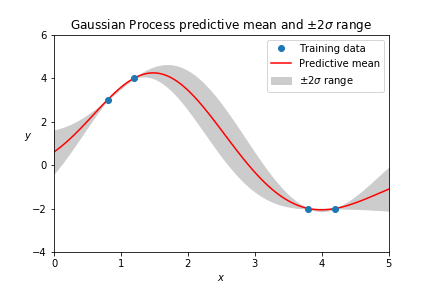
\includegraphics{gaussian_process}
        \end{center}

        \subsubsection{Function Space}
            In \hyperref[sec:BayesianLinearRegression]{Bayesian Linear Regression} we saw that it was a parametric form
            of learning the weight $\boldsymbol{w}$. Now instead we can consider the function space view were we can
            instead directly learn the function $f(\boldsymbol{x}) = \boldsymbol{w}^T\phi(\boldsymbol{x})$. We can
            express this function space view as:

            \begin{itemize}
                \item Prior: $P(f(\boldsymbol{x}_*)) = \int_{\boldsymbol{w}} P(f|\boldsymbol{w}, \boldsymbol{x}_*) P(\boldsymbol{w}))d\boldsymbol{w}$
                \item Posterior: $P(f(\boldsymbol{x}_*)|\boldsymbol{X}, \boldsymbol{y}) = \int_{\boldsymbol{w}}
                P(f|\boldsymbol{w}, \boldsymbol{x}_*) P(\boldsymbol{w}|\boldsymbol{X}, \boldsymbol{y})d\boldsymbol{w}$
            \end{itemize}

            According to every function view, there is a Gaussian at $f(\boldsymbol{x}_*)$ for every $\boldsymbol{x}_*$.
            Those Gaussians are correlated through $\boldsymbol{w}$.
            
        \subsubsection{Representation}
            We can represent a Gaussian Process, a distribution over functions as:
            $$ f(\boldsymbol{x}) \sim GP(m(\boldsymbol{x}), k(\boldsymbol{x}, \boldsymbol{x}')) \forall \boldsymbol{x},
            \boldsymbol{x}' $$

            where $ m(\boldsymbol{x}) = E(f(\boldsymbol{x})) $ is the mean and $k(\boldsymbol{x}, \boldsymbol{x}') =
            E((f(\boldsymbol{x} - m(\boldsymbol{x})))(f(\boldsymbol{x}')-m(\boldsymbol{x}')))$ is the kernel covariance
            matrix.
        
        \subsubsection{Gaussian Process Regression}
            The gaussian process regression is the kernel version of \hyperref[sec:BayesianLinearRegression]{Bayesian
            Linear Regression} where we learn based on the function space view, computing the posterior over $f$ rather
            than over $w$. This allows for the complexity to be cubic in the number of training points rather than the
            number of features. We can perform regression using the following formulae.

            Prior: $P(f(\cdot)) = N(m(\cdot),k(\cdot,\cdot))$
            
            Likelihood: $P(\boldsymbol{y}|\boldsymbol{X},f) = N(f(\cdot), \sigma^2 \boldsymbol{I})$

            Posterior: $P(f(\cdot)|\boldsymbol{X},\boldsymbol{y}) = N(\overline{f}(\cdot), k'(\cdot, \cdot))$ where \\
            $\overline{f}(\cdot) = k(\cdot,\boldsymbol{X})(\boldsymbol{K}+\sigma^2\boldsymbol{I})^{-1}\boldsymbol{y}$ and \\
            $k'(\cdot,\cdot)=k(\cdot,\cdot)-k(\cdot,\boldsymbol{X})(\boldsymbol{K}+\sigma^2\boldsymbol{I})^{-1}k(\boldsymbol{X},\cdot)$
            
            Prediction: $P(\boldsymbol{y}_*|\boldsymbol{x}_*, \boldsymbol{X}, \boldsymbol{y}) = N(\overline{f}(\boldsymbol{x}_*), k'(\boldsymbol{x}_*, \boldsymbol{x}_*))$

    \subsection{Support Vector Machines} \label{sec:SVM}
            Support Vector Machines is a kernel based method that can be used for classification and regression. It
            performs extremely well for small amounts of data and can even beat out Neural Networks. 
            \vspace{1em}
            \begin{center}
                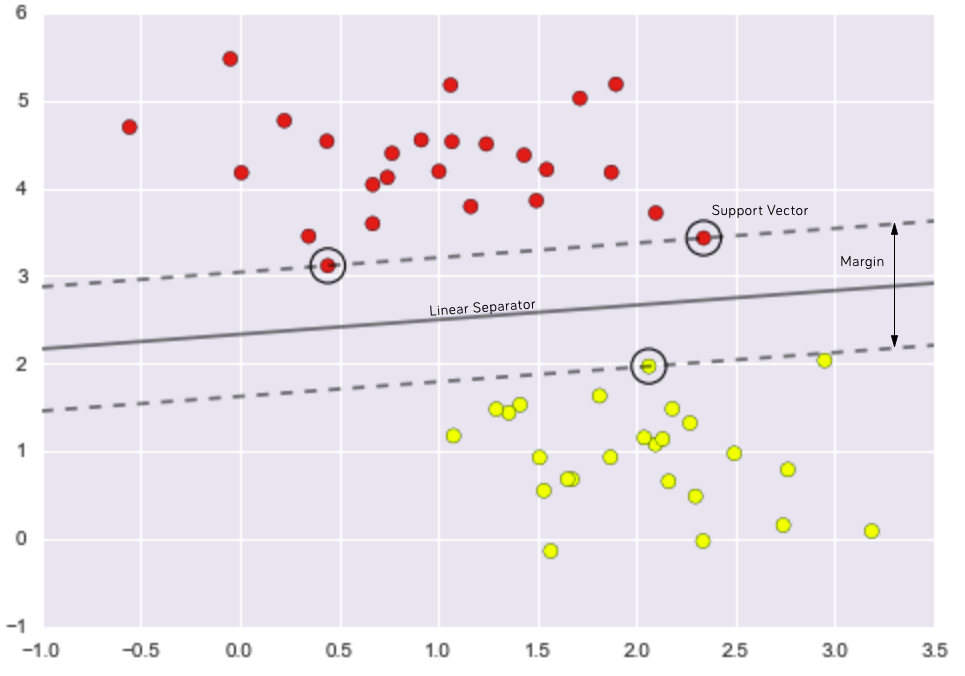
\includegraphics[scale=0.35]{SVM}
            \end{center}
        
        \subsubsection{Max-Margin Classifier}
            Max-Margin classifier is generally only used for binary classification where the data is linearly
            separable. The intuition behind the max-margin classifier is that we want to find a linear separator for
            the data that maximizes the distance to the closest data points. We formulate this method as we need to
            consider noise, a larger margin will allow room for noise, otherwise if it is too narrow then there is
            room for possible misclassification.

            We can turn the problem into an optimization problem of finding the max margin as follows.

            Linear Separator: $\boldsymbol{w}^T\phi(\boldsymbol{x}) = 0$.

            Distance to Linear Separator:
            $$ \frac{y\boldsymbol{w}^T\phi(x)}{\|\boldsymbol{w}\|}, y \in \{-1, 1\} $$

            Maximum Margin:
            $$ max_{\boldsymbol{w}} \frac{1}{\|\boldsymbol{w}\|} \{min_n y_n
            \boldsymbol{w}^T\phi(\boldsymbol{x}_n)\} $$

            We can transform this expression by fixing the minimal distance to 1 and minimizing our scale
            $\|\boldsymbol{w}\|$ to be:

            $$ min_w \frac{1}{2} \|\boldsymbol{w}\|^2 \ \ \text{s.t.} \  y_n \boldsymbol{w}^T\phi(\boldsymbol{x}_n)
            \geq 1 \ \forall n $$

            This now becomes a convex quadratic optimization problem with linear constraints, which is a form of
            that is quite easy. The points where $y_n \boldsymbol{w}^T\phi(\boldsymbol{x}_n) = 1$ define the active
            constraints, called the support vectors.

            \paragraph{Dual Representation}
                To compute this problem we want to reformulate such that $\phi(\boldsymbol{x})$ only appears in a
                kernel. From the kernel trick we see we can achieve this by finding the dual of the optimization.
                This will result in a sparse kernel since only the points on the margin matter.

                We want to transform the constrained optimization problem
                $$ min_w \frac{1}{2} \|\boldsymbol{w}\|^2 \ \ \text{s.t.} \  y_n
                \boldsymbol{w}^T\phi(\boldsymbol{x}_n) \geq 1 \ \forall n $$

                into an unconstrained optimization problem. We can use the lagrangian to obtain the following.
                $$ max_{a \geq 0} \ min_{\boldsymbol{w}} L(\boldsymbol{w}, \boldsymbol{a}) $$
                where
                $$ L(\boldsymbol{w}, \boldsymbol{a}) = \frac{1}{2} \| \boldsymbol{w} \|^2 - \sum_n a_n[y_n
                \boldsymbol{w}^T \phi(\boldsymbol{x}_n) - 1] $$
                where the second term is the penalty for violating the $n^th$ constraint.

                We can then solve the inner minimization $min_{\boldsymbol{w}}L(\boldsymbol{w}, \boldsymbol{a})$ to
                obtain:
                $$L(\boldsymbol{a}) = \sum_n a_n - \frac{1}{2}\sum_n \sum_n a_n a_n, y_n y_n, k(\boldsymbol{x}_n, \boldsymbol{x}_n)$$

                We are then left with the optimization problem in $\boldsymbol{a}$ only known as the dual problem.
                $$ max_{\boldsymbol{a}}L(\boldsymbol{a}) \ \text{s.t.} \ a_n \geq 0 $$
                This is sparse optimization since many of the $a_n$'s are 0 when the data point is already $\geq 1$,
                so the penalty is 0 for theses since they already satisfy the constraint.
                
            \paragraph{Classification}
                Primal Problem:
                $$ y_* = sgn(\boldsymbol{w}^T\phi(\boldsymbol{x}_*)) $$

                Dual Problem:
                \begin{align*}
                y_* &= sgn(\sum_n a_ny_n\phi(\boldsymbol{x}_n)^T\phi(\boldsymbol{x}_*)) \\
                y_* &= sgn(\sum_n a_ny_n k(\boldsymbol{x}_n, \boldsymbol{x}_*))
                \end{align*}
                
                Intuitively what is happening here is we are taking the sum of the degree of similarity between each
                query point and every point in the training set that is a support vector.
            
        \subsubsection{Soft Margin Classifier}
            Often times the data is not linearly separable and we have overlapping class distributions. We want a method
            such that we can relax the constraints yet keep the maximum margin as maximizing the margin is equivalent to
            minimizing an upper bound on the worst case loss. To achieve this we introduce Soft Margins which formulates
            that we can relax the constraints by introducing a slack variable $\xi \geq 0$. We can now impose the
            following constraint.
            $$ y_n \boldsymbol{w}^T\phi(\boldsymbol{x}_n) \geq 1 - \xi_n \ \forall n $$

            This introduces a new optimization problem
            $$ min_{\boldsymbol{w}, \boldsymbol{\xi}} \ C \sum_{n=1}^N \xi_n + \frac{1}{2} \| \boldsymbol{w} \|^2
            \quad \textrm{s.t.} \ y_n \boldsymbol{w}^T \phi(\boldsymbol{x}_n) \geq 1 - \xi_n, \ \xi_n \geq 0 \ \forall n
            $$
            
            $C > 0$ controls the tradeoff between the slack variable penalty and the margin. 
            
            
            Some intuition behind this is further explored. 
            \begin{itemize}
                \item Since $\sum_n \xi_n$ is an upper bound on the number of 
                misclassifications, $C$ can also be thought as a regularized coefficient that controls the tradeoff between 
                error minimization and model complexity
                \item We can see that if we let $C \rightarrow \infty$ then we recover the
                original hard margin problem.
                \item Soft margins can only handle minor misclassifications and are still sensitive 
                to outliers.
            \end{itemize}        
        
        
        \subsubsection{Multiclass SVM}
            There are many approaches to train multi class SVM's the best one being the continuous ranking approach. The
            idea behind this, is that instead of computing the sign of a linear separator, we compare the values of linear
            functions for each class $k$. The SVM returns a continuous value to rank all classes.

            \paragraph{Constraint}
            Now for each class $k \neq y$ we define a linear constraint that guarantees a margin of at least 1 between classes.
            $$ \boldsymbol{w}^T_y \phi(\boldsymbol{x}) - \boldsymbol{w}^T_k\phi(\boldsymbol{x}) \geq 1 \ \forall k \neq
            y $$

            \paragraph{Classification}
            With the constraint we can achieve the optimization problem used for classification. For multiclass dataset
            that is linearly separable we get:

            $$ min_{\boldsymbol{w}} \frac{1}{2} \sum_k \|\boldsymbol{w}_k \|^2 \quad \textrm{s.t.} \
            \boldsymbol{w}^T_{y_n} \phi(\boldsymbol{x_n}) - \boldsymbol{w}^T_k \phi(\boldsymbol{x}_n) \geq 1 \ 
            \forall n,k \neq y_n $$

            For overlapping classes we can add the slack variable $\xi$
            $$ min_{\boldsymbol{w}, \boldsymbol{\xi}} \ C \sum_n \xi_n + \frac{1}{2} \sum_k \|\boldsymbol{w}_k \|^2 \quad \textrm{s.t.} \
            \boldsymbol{w}^T_{y_n} \phi(\boldsymbol{x_n}) - \boldsymbol{w}^T_k \phi(\boldsymbol{x}_n) \geq 1 - \xi_n \ 
            \forall n,k \neq y_n $$

\section{Artificial Neural Networks Primer}
    \subsection{Origins}
        The concept of a Artificial Neural Network (ANN) stems from the anatomy of the brain. They are modelled directly
        after biological neurons, a neural cell, found in the brain. Biological neurons produce short electrical
        impulses called \textit{action potentials} which travel along the neurons and make synapses release chemical
        signals called \textit{neurotransmitters}. When a neuron receives a sufficient amount of these neurotransmitters
        within a few milliseconds, it fires its own electrical impulses. These, individual neurons behave in a simple
        way but they are organized in a vast network of billions, with each neuron typically connect to thousands of
        other neurons. Highly complex computations can be performed by a network of fairly simple neurons.

    \subsection{ANN Unit}
        Now the idea behind Artificial Neural Networks is to mimic the brain by making Artificial Neurons. The
        Perceptron is one of the simplest ANN architectures and is based on a slightly different artificial neuron
        called a \textit{threshold logic unit} (TLU), or sometimes a \textit{linear threshold unit} (LTU). The TLU
        computes a weighted sum of its inputs ($a = w_1x_1 + w_2x_2 + ... + w_nx_n = \boldsymbol{w}^T\boldsymbol{x}$),
        then applies an \hyperref[sec:ActivationFunction]{activation function} to that sum and outputs the result:
        $h_{\boldsymbol{w}}(a)$. When picking an activation function, it should be nonlinear, otherwise the network is
        just a linear function. The activation function should be chosen such that it mimics firing in neurons: the unit
        should be "active" (output near 1) when fed with the "right" inputs and the unit should be "inactive" (output
        near 0) when fed with the wrong inputs.

    \subsection{Perceptron}
        A perceptron is a type of single layer feed-forward network. It is simply composed of a single layer of threshold logic units, with each TLU connected to all the
        inputs. When all the neurons in a layer are connected to every neuron in the previous later, the layer is called
        a \textit{fully connected layer}, or a \textit{dense layer}. The inputs of the perceptron are fed to special
        pass through neurons called input neurons: they output whatever input they are fed. All the input neurons form
        the \textit{input layer}. Moreover, an extra bias feature is generally added ($x_0 = 1$): it is typically
        represented using a special type of neuron called a \textit{bias neuron}, which outputs 1 all the time.
        
        \subsubsection{Threshold Perceptron Learning}
            \paragraph{Threshold Perceptron Algorithm}
                For threshold perceptron algorithm, learning is done separately for each unit $j$ since units do not share
                weights. The learning algorithm is as follows, for each unit $j$, for each $(\boldsymbol{x},
                \boldsymbol{y})$ pair do until the output is correct for all training instances:
                \begin{itemize}
                    \item Case 1: Correct output produced then $\forall i W_{ji} \leftarrow W_{ji}$
                    \item Case 2: Output produced 0 instead of 1 then $\forall i W_{ji} + x_i$
                    \item Case 3: Output produced is 1 instead of 0 then $\forall i W_{ji} - x_i$ 
                \end{itemize}

                Now we will demonstrate the intuition behind this. If we consider using a threshold activation function then
                the perceptron computes:
                \begin{itemize}
                    \item 1 when $\boldsymbol{w}^T\overline{\boldsymbol{x}} = \sum_i x_iw_i + w_0 > 0$
                    \item 0 when $\boldsymbol{w}^T\overline{\boldsymbol{x}} = \sum_i x_iw_i + w_0 < 0$
                \end{itemize}

                Now leveraging the fact that $\overline{\boldsymbol{x}}^T\overline{\boldsymbol{x}} \geq 0$ and
                $\overline{\boldsymbol{x}}^T\overline{\boldsymbol{x}} \leq 0$ then we can we can come up with the following
                statements. 
                \begin{itemize}
                    \item If the output should be 1 instead of 0 then $\boldsymbol{w} \leftarrow \boldsymbol{w} +
                    \overline{\boldsymbol{x}}$ since $(\boldsymbol{w} + \overline{\boldsymbol{x}})^T\overline{\boldsymbol{x}}
                    \geq \boldsymbol{w}^T\overline{\boldsymbol{x}}$
                    \item If the output should be 0 instead of 1 then $\boldsymbol{w} \leftarrow \boldsymbol{w} -
                    \overline{\boldsymbol{x}}$ since $(\boldsymbol{w} - \overline{\boldsymbol{x}})^T\overline{\boldsymbol{x}}
                    \leq \boldsymbol{w}^T\overline{\boldsymbol{x}}$
                \end{itemize}
            
            \paragraph{Sequential Gradient Descent Algorithm}
                Alternatively we can use \hyperref[sec:GD]{gradient descent} to minimize misclassification error to
                train the perceptron. 

                Let $y \in \{-1, 1\} \forall y$ and let $M = \{(\boldsymbol{x}_n, y_n)_{\forall n}\}$ be the set of
                misclassified examples (i.e., $y_n \boldsymbol{w}^T\overline{\boldsymbol{x}}_n < 0$).

                We need to find a $\boldsymbol{w}$ that minimizes the misclassification error
                $$ E(\boldsymbol{w}) = -\sum_{(\boldsymbol{x}_n, y_n)\in M} y_n
                \boldsymbol{w}^T\overline{\boldsymbol{x}}_n $$
                and the gradient is:
                $$ \boldsymbol{\nabla E} = -\sum_{(\boldsymbol{x}_n, y_n)\in M} y_n \overline{\boldsymbol{x}}_n $$

                Now applying this to the gradient descent algorithm we have:
                $$ \boldsymbol{w} \leftarrow \boldsymbol{w} + \alpha y \overline{\boldsymbol{x}} $$
                We adjust $\boldsymbol{w}$ one sample at a time. Here $\alpha$ is the learning rate and we see that if
                we let $\alpha = 1$ then we recover the threshold perceptron algorithm.
            
            \paragraph{Limitations}
                The decision boundary of each output neuron is linear, so Perceptrons are incapable of learning complex
                However, if the training instances are linearly separable then this algorithm will converge to a solution.
        
        \subsubsection{Sigmoid Perceptron Learning}
            Similar to Threshold perceptron learning, Sigmoid Perceptron Learning hinges on the same concepts. We can
            set our objective to minimizing the minimum squared error or maximum likelihood which will yield the same
            algorithm as for \hyperref[sec:LogisticRegression]{logistic regression}. 
            $$ E(\boldsymbol{w}) = \frac{1}{2} \sum_n E_n (\boldsymbol{w})^2 = \frac{1}{2} \sum_n (y_n -
            \sigma(\boldsymbol{w}^T\overline{\boldsymbol{x}}_n))^2 $$

            We can compute the gradient to be
            $$ \boldsymbol{\nabla E} = -\sum_n E_n(\boldsymbol{w})\sigma(\boldsymbol{w}^T
            \overline{\boldsymbol{x}}_n)(1-\sigma(\boldsymbol{w}^T \overline{\boldsymbol{x}}_n))x_i $$

            Now using sequential gradient descent we repeat the following for each $(\boldsymbol{x}_n, y_n)$ until some
            stopping criterion is satisfied. 
            $$ \epsilon_n \leftarrow y_n - \sigma(\boldsymbol{w}^T \overline{\boldsymbol{x}}_n) $$
            $$ \boldsymbol{w} \leftarrow \boldsymbol{w} + \alpha \epsilon_n \sigma(\boldsymbol{w}^T
            \overline{\boldsymbol{x}}_n) (1 - \sigma(\boldsymbol{w}^T
            \overline{\boldsymbol{x}}_n))\overline{\boldsymbol{x}}_n $$

            It possesses the same limitations as threshold perceptron learning.

    \subsection{Multi-Layer Neural Nets}
        We previously saw the limitations of the perceptron as it was only able to learn on linearly separable data.
        Unfortunately a lot of data is not linear and this led to the birth of Multi-layer Neural Networks:
        which are able to learn non-linear basis functions.

        \subsubsection{n-Layer Perceptron}
            The follow diagram depicts a 2 layer perceptron. Multilayer perceptron are composed of one (passthrough)
            \textit{input layer}, one or more layers of ANN's units called \textit{hidden layers}, and one final layer of
            ANN units called the \textit{output layer}. The layers close to the input layer are usually called the
            \textit{lower layers}, and the ones close to the outputs are usually called the \textit{upper layers}. Every
            layer except the output layer includes a bias neuron and is fully connected to the next layer.
            
            \begin{center}
                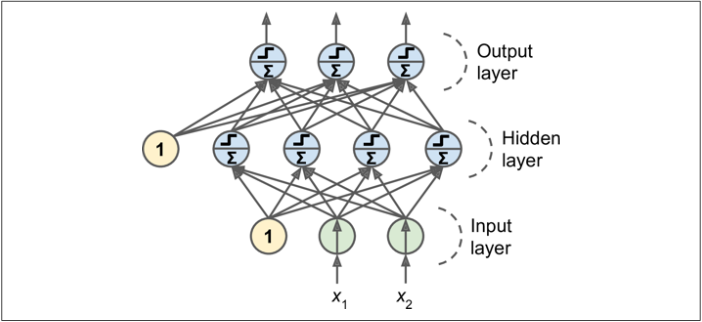
\includegraphics[scale=0.65]{MLP}
            \end{center}

            Let us denote the hidden units with $\boldsymbol{z}$, the output units with $\boldsymbol{y}$ and the weights
            between the layers with $\boldsymbol{w}^(layer_num)$.
            
            Hidden Units: $z_j = h_1(\boldsymbol{w}_j^{(1)} \overline{\boldsymbol{x}})$

            Output Units: $y_k = h_2(\boldsymbol{w}_k^{(2)} \overline{\boldsymbol{z}})$

            Overall: $y_k = h_2 (\sum_j w_{kj}^{(2)} h_1(\sum_i w_{ji}^{(1)}x_i))$

            \paragraph{Non-linear Regression}
                We can use a multi-layer neural network to equivalently represent regression with the following expression.
                $$ y_k = \sum_j w_{kj}^{(2)} \sigma(\sum_i w_{ji} x_i) $$

                We can interpret the \hyperref[sec:Sigmoid]{sigmoid} as a non linear basis function and the outer summation to be the linear
                combination. 
                
            \paragraph{Non-linear Classification}
                We can use a multi-layer neural network to equivalently represent binary classification with the following
                expression.
                $$ P(c_k | \boldsymbol{x}) = \sigma(\sum_j w_{kj}^{(2)} \sigma(\sum_i w_{ji} x_i)) $$
                
                We can interpret the \hyperref[sec:Sigmoid]{sigmoid} as a non-linear basis function and the outer summation to be the linear
                combination. The outer sigmoid is the normalization to return the probability.

            What is happening in both regression and classification is we are allowing the basis functions to adapt and
            vary and we are no longer restricted to fixed basis functions.
        
        \subsubsection{Backpropagation} \label{sec:Backprop}
            One of the most common forms of weight training for multi-layer neural nets is error minimization using
            backpropagation. This allows us to compare the errors at the output and backpropagate the error
            back through the error through the network to train the weights.

            We can then use \hyperref[sec:GD]{gradient descent} to to adjust the weights. Generally based on the size of
            the model and the data it is more favorable to use faster gradient descent algorithms and we can consider
            \hyperref[sec:GDO]{gradient descent optimizations} for training.

            \paragraph{Algorithm}
                Forward Phase: Propagate units forward to compute the output of each unit. We want to obtain the output
                $z_j$ for each unit $j$.
                $$ z_j = h(a_j) \quad \text{where} \quad a_j = \sum_i w_{ji} z_i $$

                Backward Phase: compute delta $\delta_j$ at each unit $j$. We can use chain rule to recursively compute
                the gradient and follow the following process.
                
                For each weight $w_{ji}$
                $$ \frac{\partial E_n}{\partial w_{ji}} = \frac{\partial E_n}{\partial a_{j}} \frac{\partial
                a_j}{\partial w_{ji}} = \delta_{j} z_i $$ 

                Let $\delta_j = \frac{\partial E_n}{\partial a_{j}}$ then
                \[ \delta_j = \begin{cases} 
                    h'(a_j)(z_j - y_j) & \text{base case: $j$ is an output unit} \\
                    h'(a_j)\sum_k w_k \delta_k & \text{recursion: $j$ is a hidden unit}
                    \end{cases}
                \]
                
                Since $a_j = \sum_i w_{ji}z_i$ then $\frac{\partial a_j}{\partial w_{ji}} = z_i$.

\section{Deep Learning}
    A Deep Neural Network is a neural network with many hidden layers. The main advantage of a DNN is its high
    expressivity, it is able to learn very complex underlying functions. As we increase the number of layers, the number
    of ANN units needed may decrease (with the number of layers). The power and basis of deep learning is that instead
    of having to have domain knowledge about what features to apply machine learning to, deep neural networks are able
    to learn hierarchical feature representations. For example for facial classification the first hidden layer detects
    certain strokes, the next is able to detect facial features such as eyes and noses and so on until it is able to
    reconstruct and detect the face.
    
    \subsection{Vanishing/Exploding Gradients Problem} \label{sec:VanishingProblem}
        One of the problems of \hyperref[sec:Backprop]{backpropagation} in deep neural networks consisting of sigmoid
        and hyperbolic units is that they often suffer from \textit{vanishing gradients}. The problem here is that the
        computed gradients get smaller and smaller as the algorithm progresses down to the lower layers. As a result,
        the \hyperref[sec:GD]{gradient descent} update leaves the lower layers' connection weights virtually unchanged,
        and training never converges to a good solution. This is because when moving in the forward phase the
        variance keeps increasing after each layer until the activation saturates at the top layer when using the
        \hyperref[sec:Sigmoid]{sigmoid} or \hyperref[sec:Tanh]{tanh} activation function. When the function
        saturates at 0 or 1, with a derivative extremely close to 0, then when backpropagation kicks in it has
        virtually no gradient to propagate back through the network. The little gradient that exists keeps getting
        diluted as backpropagation progresses down through the top layers, so there is really nothing left for the
        lower layers.
        
        Some popular solutions for this problem are:
        \begin{itemize}
            \item Pre-training
            \item \hyperref[sec:reLU]{Recfitified Linear Units} and \hyperref[sec:MaxoutUnits]{Maxout Units}
            \item \hyperref[sec:ResNet]{Residual Networks/Skip Connections}
            \item \hyperref[sec:BatchNormalization]{Batch Normalization}
        \end{itemize}

        \subsubsection{Batch Normalization} \label{sec:BatchNormalization}
            Although using the \hyperref[sec:reLU]{reLU} activation function can reduce the danger of
            vanishing/exploding gradient problem, it doesn't guarantee that it won't come back. Batch Normalization
            addresses this problem. The technique consists of adding an operation in the model just before or after the
            activation function of each hidden layer. This operation simply zero-centers and normalizes each input, then
            scales and shifts the result using two new parameter vectors per layer: one for scaling, the other for
            shifting. The operations lets the model learnt the optimal scale and mean of each of the layer's inputs. In
            many cases if you add a BN layer as the very first layer of your neural network, you do not need to
            standardize your training set; the BN will do it for you. 

            In order to zero-center and normalize the inputs, the algorithm needs to estimate each input's mean and
            standard deviation. It does so by evaluating the mean and standard deviation fo the input over the current
            mini-batch.
            
            When testing the trained network we need to make predictions for individual instances rather than for
            batches of instances: in this case, we have no way to compute each input's mean and standard deviation. One
            solution is to wait till the end of training and run the whole training set through the neural network and
            compute the mean and standard deviation of each input of the BN layer. However, most implementations of
            Batch Normalization estimate these final statistics during training by using a moving average of the layer's
            input means and standard deviations.

            Batch Normalization does, however, add some complexity to the model. Moreover there is a runtime penalty:
            the neural network makes slow predictions due to the extra computations required at each layer. Fortunately,
            it's often possible to fuse the BN layer with the previous layer, after training, thereby avoiding the
            runtime penalty. This is done by updating the previous layer's weights and biases so that it directly
            produces outputs of the appropriate scale and offset.

        \subsubsection{Residual Networks} \label{sec:ResNet}
            Even with \hyperref[sec:reLU]{reLU}, very deep networks suffer from vanishing gradients. Residual Networks
            leverages an architecture with sip connections, which are essentially connections from early layers to later
            layers bypassing certain layers. In Residual Networks the input $\boldsymbol{x}$ of the skip connection is added to the
            output of the layers it skipped thus the overall output is $f(\boldsymbol{x}) + \boldsymbol{x}$. The
            intuition behind this type of skip connection sit that they have an uninterrupted gradient flow from the
            first layer to the last layer. If the output of some combination of layers results in a gradient of almost
            then by using skip connections we pass the original input $x$ to the output, allowing us to use that
            gradient rather than the diminished one.

            \begin{center}
                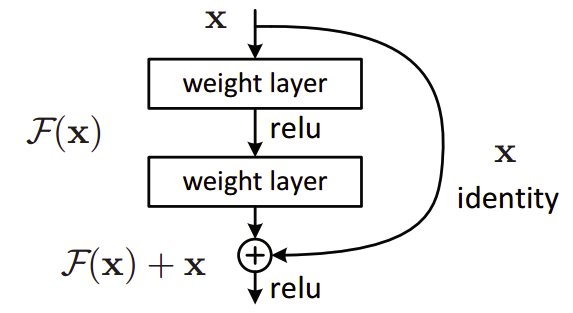
\includegraphics[scale=0.5]{ResNet.png}
            \end{center}

    \subsection{Overfitting}
        Since deep neural networks are so highly expressive this increases the risk of overfitting. Often times the
        number of parameters is larger than the amount of data. We can use some of the follow techniques to help
        mitigate overfitting.
    
        \begin{itemize}
            \item \hyperref[sec:Regularization]{Regularization}
            \item \hyperref[sec:Dropout]{Dropout}
            \item \hyperref[sec:DataAugmentation]{Data augmentation}
        \end{itemize}

        \subsubsection{Dropout} \label{sec:Dropout}
            The idea behind dropout is to randomly "drop" some units from the network when training, this effectively is
            the same as saying to reduce their values to 0. Now we train the model with missing nodes (that could
            represent features) making the network robust if it is able to still perform well and making it impervious
            to overfitting since it can perform well with some features removes. In each training iteration, a different
            subnetwork is trained. At test time, these subnetworks are merged by averaging their weights.

            At training during each iteration of gradient descent:
            \begin{itemize}
                \item Each input unit is dropped with probability $p_1$
                \item Each hidden unit is dropped with probability $p_2$.
            \end{itemize}

            For prediction, since we scaled down the inputs by probability $p_1$ and the hidden units by $p_2$, so we need to
            multiply by their complementary probability to increase their magnitude accordingly.
            \begin{itemize}
                \item Multiply each input unit by $1 - p_1$
                \item Multiply each hidden unit by $1 - p_2$
            \end{itemize}

            \paragraph{Algorithm}
            Let $\odot$ denote elementwise multiplication.
            For each training example $(\boldsymbol{x}_n, y_n)$ do
            \begin{align*}
                & \text{Sample} \; \boldsymbol{z}_n^{(1)} \; \text{from Bernoulli} (1 - p_i)^{k_i} \; \text{for} \; 1 \leq l \leq L \\
                & \text{Neural Network with dropout applied: } \\ 
                & f_n(\boldsymbol{x}_n, \boldsymbol{z}_n; \boldsymbol{W}) = h_i(\boldsymbol{W}^{(L)} [...h_2(\boldsymbol{W}^{(2)}[h_1(\boldsymbol{W}^{(1)}[\overline{\boldsymbol{x}}_n \odot \boldsymbol{z}_n^{(1)}])\odot \boldsymbol{z_n}^{(2)}])... \odot \boldsymbol{z}_n^{(L)}]) \\
                & \text{Loss: } \; Err(y_n, f_n(\boldsymbol{x}_n, \boldsymbol{z}_n; \boldsymbol{W})) \\
                & \text{Update: } \; w_{kj} \leftarrow w_{kj} - \alpha \frac{\partial Err}{\partial w_{kj}}
            \end{align*}
            Until convergence.

            Prediction:
            $$ f(\boldsymbol{x}_n; \boldsymbol{W}) = h_i(\boldsymbol{W}^{(L)}
            [...h_2(\boldsymbol{W}^{(2)}[h_1(\boldsymbol{W}^{(1)}[\overline{\boldsymbol{x}}_n (1-p_1)])(1-p_2)])...
            (1-p_L)]) $$        
        
        \subsubsection{Data Augmentation} \label{sec:DataAugmentation}
            Data augmentation artificially increases the size of the training set by generating many realistic variants
            of each training instance. This reduces overfitting, making this a possible regularization technique. The
            generated instances should be as realistic as possible,: ideally, given an image from the augmented
            training set, a human should not be able to tell whether it was augmented or not. 

            Some data augmentation methods are things like, slightly shifting, rotating or resizing every picture in the
            training set by various amounts and add the resulting pictures to the training set. This forces the model to
            be more tolerant to variations in the position, orientation, and size of the objects in the pictures. You
            can also play around with lighting and flip the pictures horizontally. By combining these transformations,
            you can greatly increase the size of your training set.

\section{Convolutional Neural Networks} \label{sec:CNN}
    Convolutional networks are a specialized king of neural network for processing data that has a known grid-like
    topology. Examples include time-series data, which can be thought of as a 1-D grid taking samples at regular time
    intervals, and image data, which can be thought of as a 2-D grid of pixels. 

    \subsection{Convolution}
        In its most general form, convolution is a mathematical operation on two functions of real-valued argument. In
        essence it uses a weighted function $w(\tau)$, where $\tau$ is the age of the measurement. It applies this weight
        average operation at every moment to obtain a new function $y$ providing a smoothed estimate of the original
        function $x$.
        $$ y(t) = \int_t x(\tau)w(t - \tau)d\tau $$

        This is the convolution and it is typically denoted with an asterisk.
        $$ y(t) = (x * w)(t) $$

        In convolutional network terminology, the first argument ($x$) to the convolution is referred to as the \textit{input},
        and the second argument ($w$) as the \textit{kernel}. The output is sometimes referred to as the \textit{feature
        map}.

        Often times we will be working with discretized data and we can define the discrete convolution as:
        $$ y(t) = (x * w)(t) = \sum_{\tau = -\infty}^{\infty} x(\tau)w(t-\tau) $$

        In machine learning applications, the input is usually a multidimensional array of data, and the kernel is
        usually a multidimensional array of parameters that are adapted by the learning algorithm. For this we often
        require to use convolutions over more than one axis at a time. In this case we would want to use a
        two-dimensional kernel K and express the convolution as:
        $$ y(i,j) = (I * K)(i,j) = \sum_m \sum_n I(m, n)K(i-m,j-n) $$
        and by commutativity:
        $$ y(i,j) = (I * K)(i,j) = \sum_m \sum_n I(i-m, j-n)K(m,n) $$

        Many neural network libraries will also implement a related function called the \textit{cross-correlation},
        which is that same as convolution but without flipping the kernel:
        $$ y(i,j) = (I * K)(i,j) = \sum_m \sum_n I(i+m, j+n)K(m,n) $$
    
        \subsubsection{Convolutions for Feature Extraction}
            In neural networks a convolution denotes the linear combination of a subset of units based on a specific
            pattern of weights. 
            $$ a_j = \sum_i w_{ji}z_i $$

            Convolutions are often combined with an activation function to produce a feature
            $$ z_j = h(a_j) = h(\sum_i w_{ji}z_i) $$
    
    \subsection{Architecture}
        The architecture of a CNN refers to any network that includes an alternation of convolution and pooling layers,
        where some of the convolution weights are shared.
                
        \subsubsection{Filters}
            A neuron's weights can be represented as a small image the size of the receptive field or window called
            filters. When applying a filter over a receptive field the neurons using those weights will ignore
            everything in their receptive field except for what that filter dictates. E.g a vertical filter will cause
            all neurons to ignore everything except for the central vertical line (since all inputs will get multiplied
            by 0, except for the ones located on the central vertical line). A layer full of neurons using the same
            filter outputs a feature map, which highlights the areas in an image that activate the filter the most. You
            do not have to define the filters manually, during training the convolutional layer wil automatically learn
            the most useful filters for its task.

        \subsubsection{Convolutional Layers}
            The most important building block of a CNN is the \textit{convolutional layer}, neurons in the first
            convolutional layer are not connected to every single pixel in the input image, but only to pixels in their
            receptive field. In turn each neuron in the second convolutional layer is connected only to neurons located
            within the small window in the first layer. This architecture allows the network to concentrate on small
            low-level features in the first hidden layer, then assemble them into larger higher-level features in the
            next hidden layer, and so on. For each window we apply the same filter / set of weights. 

            \begin{center}
                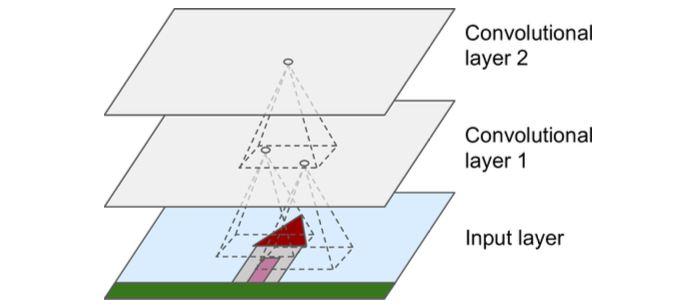
\includegraphics[scale=0.65]{ConvLayer}
            \end{center}

            It is also possible to connect a large input layer to a smaller layer by spacing out the receptive fields, which reduces the
            complexity and dimensionality. The shift from one receptive field to the next is called the stride. 
            
            \begin{center}
                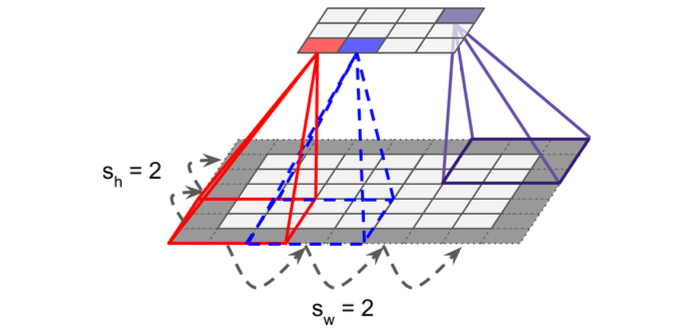
\includegraphics[scale=0.65]{ConvStride}
            \end{center}

        \subsubsection{Pooling Layers}
            The goal of pooling layers is to \textit{subsample} the input image in order to reduce the computational
            load, the memory usage, and the number of parameters (reducing risk of overfitting). Just like in
            convolutional layers, each neuron in a pooling layer is connected to the outputs of a limited number of
            neurons in the previous layer, located within a small rectangular receptive field. For each receptive field
            we must define its size, stride and padding type similar to the Convolutional Layer. The difference is that
            a pooling neuron has no weights; all it does is aggregate the inputs using an aggregation function such as
            max or mean. For example in a max pooling layer only the max value in each receptive field makes it to the
            next layer.

            The pooling layers also introduce some level of \textit{invariance} to small translations. For example when
            if you have a max pooling layer and you shift some pixels around in the receptive field the output for that
            receptive field will still be the same. 
        
        \subsubsection{Parameters}
            \begin{itemize}
                \item \textbf{Number of Filters}: integer indicating the number of filters applied to each window/receptive field.
                \item \textbf{Kernel Size}: tuple(width, height) indicating the size of the window/receptive field.
                \item \textbf{Stride}: tuple(horizontal, vertical) indicating the horizontal and vertical shift between
                each window/receptive field. 
                \item \textbf{Padding}: "valid" or "same". Valid indicates no input padding. Same indicates that the
                input is padded with a border of zeros to ensure that the output has the same size as the input.
            \end{itemize}
    
    \subsection{Benefits/Advantages}
        \subsubsection{Sparse Interactions}
            Since there are fewer connections between layers due to the organization of the receptive fields then it is
            easier to train and less computationally expensive.
        
        \subsubsection{Parameter Sharing}
            For each receptive field the same filter is applied so there are fewer weights that have to be computed also
            making it less computationally expensive and less complex.
        
        \subsubsection{Locally Equivariant Representation}
            With pooling layers we are able to make the network robust and invariant to translations as well as handle
            inputs of varying length.

\section{Hidden Markov Models}
    Hidden Markov models provide a way to make predictions for a sequence of data where the prediction for one data
    point is dependent or correlated with the prediction for the next data point. This is different than other models
    that treat each data point independently. For example in speech recognition words can be recognized/interpreted based on the
    sound of the syllables before it. Hidden Markov models are a generalization of
    \hyperref[sec:MixtureOfGaussian]{Mixture of Gaussians}.

    \begin{center}
        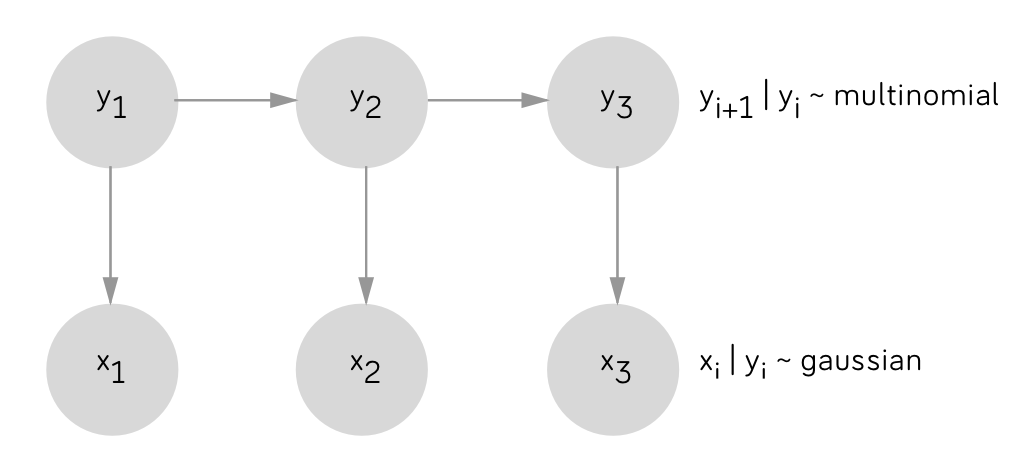
\includegraphics[scale=0.3]{HMM}
    \end{center}

    \subsection{Assumptions} 
        \subsubsection{Stationary Process}
            Transition and emission distributions are identical at each step
            \begin{align*}
                & P(x_t|y_t) = P(x_{t+1}|y_{t+1}) \; \forall t \\
                & P(y_t|y_{t-1}) = P(y_{t+1}|y_{t}) \; \forall t
            \end{align*}
        
        \subsubsection{Markovian Process}
            Next state is independent of previous states given the current statements
            $$ P(y_{t+1}|y_{t}, y_{t-1},...,y_{1}) = P(y_{t+1}|y_{t}) \; \forall t $$
        
        \subsubsection{Distributions}
            Initial Distribution
            $$ P(y_i) \sim multinomial $$

            Transition Distribution
            $$ P(y_{i+1}|y_{i}) \sim multinomial $$

            Emission Distribution
            \begin{align*}
                P(x_{t} | y_{t}) & \sim gaussian (continuous) \\
                & \sim multinomial (discrete)
            \end{align*}

            Joint Distribution
            $$ P(y_{1 .. t}, x_{1 .. t}) = P(y_{1})\prod_{i=1}^{t-1} P(y_{i+1}|y_{i}) \prod_{i=1}^{t} P(x_{i}|y_{i})
            $$
            
    \subsection{Inference in Temporal Models}
        There are many applications of Hidden Markov Models for example mobile robot localisation. 
        In scenarios like we generally want to compute 4 common tasks:
        \begin{itemize}
            \item \textbf{Monitoring: } $P(y_t|x_{1..t})$
            \item \textbf{Prediction: } $P(y_{t+k} | x_{1..t}) $
            \item \textbf{Hindsight: } $P(y_k | x_{1..t})$ where $k < t$
            \item \textbf{Most Likely Explanation: } $argmax_{y_1,...,y_t} P(y_{1..t}|x_{1..t})$
        \end{itemize}
        
        \subsubsection{Monitoring}
            $P(y_{t}|x_{1..t})$: distribution of current state given observations. We can employ recursive computation to 
            decompose the query to be in terms of the probability of the previous hidden state.

            $$ P(y_{t}|x_{1..t}) \propto P(x_t)P(y_t) \sum_{y_{t-1}}P(y_{t}|y_{t-1})P(y_{t-1}|x_{1..t-1}) $$

            Now with this derivation we can compute $P(y_{t}|x_{1..t})$ by forward computation.

            \begin{align*}
                & P(y_1|x_1) \propto P(x_1|y_1)P(y_1) \\
                & \text{For} \; i=2 \; \text{to} \; t \; \text{do} \\
                & \qquad P(y_{i}|x_{1..i}) \propto P(x_i|y_i)\sum_{y_{i-1}} P(y_{i}|y_{i-1})P(y_{i-1}|x_{1..i-1}) \\
                & \text{End}
            \end{align*}

            Linear complexity in $t$
        
        \subsubsection{Prediction}
            $P(y_{t+k}|x_{1..t})$: distribution over future state up to $k$ given observations. Using recursive
            computation we obtain
            $$ P(y_{t+k}|x_{1..t} = \sum_{y_{t+k-1}} P(y_{t+k} | y_{t+k-1})P(y_{t+k-1}|x_{1..t}) $$
            where we predict based on the previous state.

            Now computing $P(y_{t+k} | x_{1..t})$ by forward computation, we first have to use monitoring until we
            need to do prediction.
            \begin{align*}
                & \text{For} \; j=1 \; \text{to} \; k \; \text{do} \\
                & \qquad P(y_{t+j}|x_{1..t}) = \sum_{y_{t+j-1}} P(y_{t+j}|y_{t+j-1})P(y_{t+j-1}|x_{1..t}) \\
                & \text{End}
            \end{align*}

            Linear complexity in $t+k$.
        
        \subsubsection{Hindsight}
            $P(y_k|x_{1..t})$ for $k < t$: distribution over a paste state give observations. Some examples of this
            are delayed activity/speech recognition.

            Computation:
            $$ P(y_k|x_{1..t}) = P(y_k|x_{1..k})P(x_{k+1..t}|y_k) $$
            We see this is composed of two parts the first being the forward monitoring and the latter being the 
            backward part where we take the future observations and propagate them back. The latter can be expressed as:
            $$ P(x_{k+1..t}|y_k) = \sum_{y_{k+1}} P(y_{k+1}|y_k) P(x_{k+1}|y_{k+1})P(x_{k+2..t}|y_{k+1}) $$

            The algorithm for computation is the forward-backward algorithm expressed as follows.
            
            1. Compute $P(y_k|x_{1..k})$ by forward computation (monitoring)

            2. Compute $P(x_{k+1..t}|y_k)$ by backward computation
            \begin{align*}
                & P(x_t|y_{t-1}) = \sum_t P(y_t|y_{t-1})P(x_t|y_t) \\
                & \text{For} \; j=t-1 \; \text{downto} \; k \; \text{do} \\
                & \qquad P(x_{j..t}|y_{j-1}) = \sum_{y_j} P(y_j|y_{j-1}) P(x_{j}|y_{j})P(x_{j+1..t}|y_{j}) \\
                & \text{End}
            \end{align*}
            
            3. $P(y_k|x_{k+1..t}) \propto P(y_k|x_{1..k})P(x_{k+1..t}|y_k)$

            Linear complexity in $t$.
        
        \subsubsection{Most Likely Explanation}
            $argmax_{y_{1..t}} P(y_{1..t}|x_{1..t})$: most likely state sequence given observations.

            Computation:
            $$ max_{y_{1..t}} P(y_{1..t}|x_{1..t}) = max_{y_t} P(x_t|y_t) max_{y_{1..t-1}} P(y_{1..t}|x_{1..t-1}) $$

            By Recursive Computation we get:
            $$ max_{y_{1..i-1}} P(y_{1..i}|x_{1..i-1}) \propto max_{y_{i-1}} P(y_i|y_{i-1})P(x_{i-1}|y_{i-1})
            max_{y_{1..i-2}} P(y_{1..i-1}|x_{1..i-2}) $$ 
        
            Now we can use this to compute $max_{y_{1..t}} P(y_{1..t}|x_{1..t})$ by dynamic programming.

            \paragraph{Viterbi Algorithm}
                \begin{align*}
                    & max_{y_1} P(y_{1..2}|x_1) \propto max_{y_1} P(y_2|y_1)P(x_1|y_1)P(y_1) \\
                    & \text{For} \; i=2 \; \text{to} \; t-1 \; \text{do} \\
                    & \qquad max_{y_{1..i}} P(y_{1..i+1}|x_{1..i}) \propto max_{y_i} P(y_{i+1}|y_i)P(x_i|y_i) max_{y_{1..i-1}} P(y_{1..i} | x_{1..i-1}) \\
                    & \text{End} \\
                    & max_{y_{1..t}} P(y_{1..t}|x_{1..t}) \propto max_{y_t} P(x_t|y_t) max_{y_{1..t-1}} P(y_{1..t}|x_{1..t-1})
                \end{align*}
                
                Linear complexity in $t$.

\section{Recurrent Neural Networks} \label{sec:RNN}
    When posed with the problem of handling variable length data (e.g., sequences, time-series, spatial data) this poses
    a problem of a variable number of parameters. Using Recurrent Neural Networks we can handle sequences of variable
    length data, we can generalize this to handle trees and graphs using Recursive Neural Networks.

    \subsection{Recurrent Neurons}
        In Recurrent Neural Networks, the outputs can be fed back to the network as inputs, creating a recurrent
        structure that can be unrolled to handle varying length data. The simplest possible RNN, composed of one neuron
        receiving inputs, producing an output, and sending that output back to itself. At each time step $t$, this
        recurrent neuron receives the inputs $\boldsymbol{x}_t$ as well as its own output from the previous time step
        $\boldsymbol{y}_{t-1}$. Since there is no previous output at the first time step, it is generally set to 0. 

        \begin{center}
            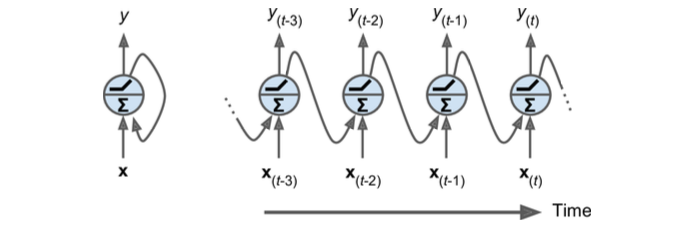
\includegraphics[scale=0.65]{RecurrentNeuron}
        \end{center}

        To create a layer of recurrent neurons. At each time step $t$, every neuron receives both the input vector $\boldsymbol{x}_t$
        and the output vector from the previous step $\boldsymbol{y}_{t-1}$. Each recurrent neuron has two sets of weights: one for
        the inputs $\boldsymbol{x}_t$ and the other for the outputs of the previous time step $\boldsymbol{y}_{t-1}$.
        call these weight vectors $\boldsymbol{w}_x$ and $\boldsymbol{w}_y$. If we consider the whole recurrent layer we
        can place all weight vectors in two weight matrices, $\boldsymbol{W}_x$ and $\boldsymbol{W}_y$. 

        The output of a recurrent layer for a single instance can be represented with the following equation where $b$
        is the bias vector and $\phi(\cdot)$ is the \hyperref[sec:ActivationFunction]{activation function}.
        $$ \boldsymbol{y}_t = \phi(\boldsymbol{W}_x^T \boldsymbol{x}_t + \boldsymbol{W}_y^T \boldsymbol{y}_{t-1} + \boldsymbol{b}) $$

        Similarly we can compute a recurrent layer's output using mini-batch by placing all the inputs at time step $t$
        in an input matrix $\boldsymbol{X}_t$.
        $$ \boldsymbol{Y}_t = \phi( \begin{bmatrix} \boldsymbol{X}_t & \boldsymbol{Y}_{t-1} \end{bmatrix} \boldsymbol{W}
        + \boldsymbol{b}) \; \text{with} \; \boldsymbol{W} = \begin{bmatrix} \boldsymbol{W}_x \\ \boldsymbol{W}_y
        \end{bmatrix} $$
        
        \subsubsection{Memory Cells}
            The output of a recurrent neuron at time step $t$ is a function of all the inputs from the previous steps,
            so it has some form of \textit{memory}. A part of neural network that preservers some state across time
            steps is called a memory cell. A single recurrent neuron, or a layer of neurons is a very basic cell,
            capable of learning only short patterns.

            In general a cell's tate at time step $t$, denoted $\boldsymbol{h}_t$, is a function of some inputs at that
            time step and its state at the previous time step: $\boldsymbol{h}_t = f(\boldsymbol{h}_{t-1},
            \boldsymbol{x}_t)$. Its output at time step $t$, denoted $\boldsymbol{y}_t$, is also a function of the
            previous state and the current inputs. In the case of basic cells the output is equal to the state, but in
            more complex cells this is not always the case.

            \begin{center}
                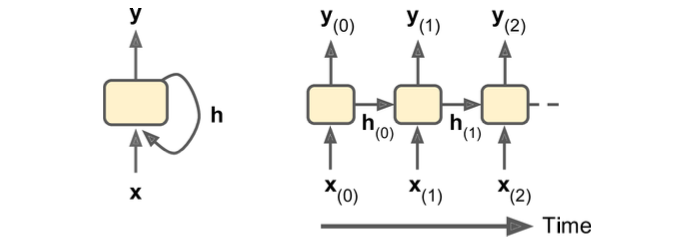
\includegraphics[scale=0.65]{MemCell}
            \end{center}
        
        \subsection{Bi-directional RNN}
            The recurrent networks we have considered up to now have a "causal" structure, meaning that the state at
            time $t$ captures only information from the past, and the present input. In many applications, however, we
            what to output a prediction of $\boldsymbol{y}_t$ that may depend on the \textit{whole input sequence}. For
            example, in speech recognition, the correct interpretations of the current sound as a phoneme may depend on
            the new fex phonemes because of co-articulation and may even depend on the next few words because of the
            linguistic dependencies between nearby words. This is also true of handwriting recognition and many other
            sequence-to-sequence learning tasks.

            Bidirectional recurrent neural networks were invented to address that need. Bidirectional RNNs combine an
            rNN that moves forward through time, beginning from the start of the sequence with another RNN that moves
            backwards through time, beginning from the end of the sequence. 
            
    \subsection{Encoder-Decoder Model}
        Often times when dealing with sequences of data the output sequence is not necessarily the same length as the
        input sequence. Additionally, sometimes the output is not always a one to one mapping with the input. A good
        example of this is language translation where translation from english to another language does not guarantee
        the sentence will be the same length or that the first word in an english sentence matches the first word in the
        output language. Here we discuss how an RNN can be trained to map an input sequence to an output sequence that
        is not necessarily of the same length.

        We often call the input to the RNN the context. We want to produce a representation of this context, $C$. The
        context $C$ might be a vector or sequence of vectors that summarize the input sequence $\boldsymbol{X}$.

        The simplest RNN architecture for mapping a variable-length sequence to another variable-length sequence is the
        encoder-decoder or sequence-to-sequence architecture. The idea is illustrated with the following items. Let
        $\boldsymbol{x}^{(i)}$ be the $i^{th}$ input and $\boldsymbol{y}^{(i)}$ by the $i^{th}$ output.

        \begin{itemize}
            \item An encoder or reader or input RNN processes the input sequence. The encoder emits the context $C$,
            as a simple function of its final hidden state.
            \item A decoder or writer or output RNN is conditioned on that fixed-length vector to generate the output
            sequence $\boldsymbol{Y} = (\boldsymbol{y}^{(1)}, ..., \boldsymbol{y}^{(n_y)})$.
        \end{itemize}

        \begin{center}
            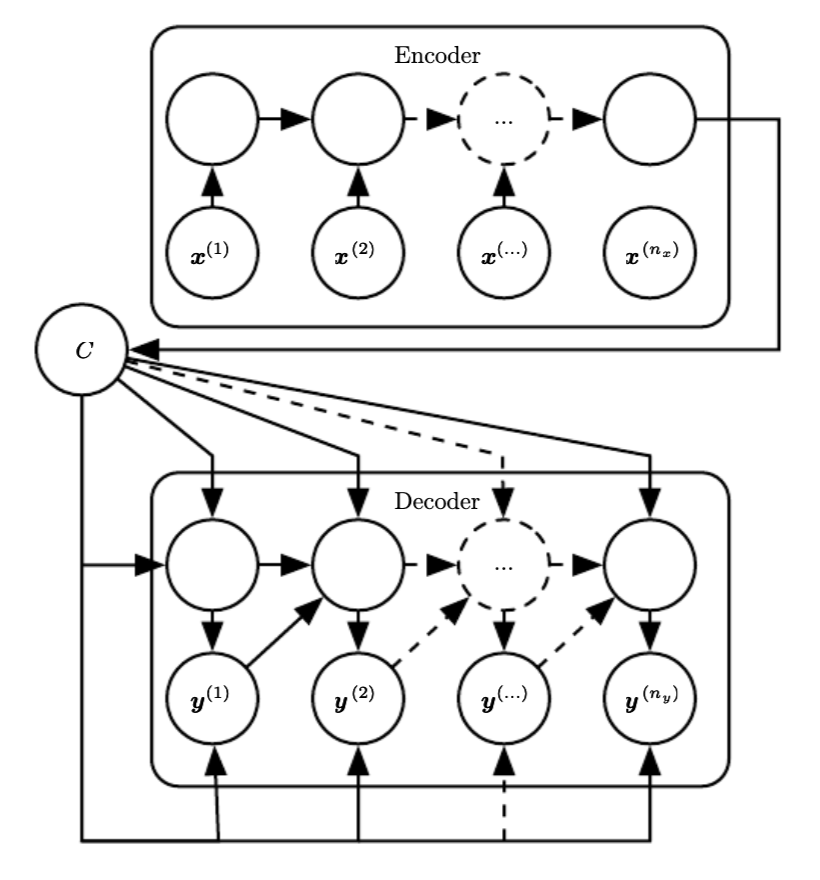
\includegraphics[scale=0.65]{encoder-decoder}
        \end{center}

        The innovation in this kind of architecture is that the lengths of the input ($n_x$) and the outputs ($n_y$)
        vary from each. Previous architectures constrained $n_x = n_y$. In a sequence-to-sequence architecture, the two
        RNNs are trained jointly to maximize the average of log $P(\boldsymbol{y}^{(1)}, ..., \boldsymbol{y}_{(n_y)}|
        \boldsymbol{x}^{(1)}, ... \boldsymbol{x}_{(n_x)})$ over all the pairs of $\boldsymbol{x}$ and $\boldsymbol{y}$
        sequences in the training set. The last state $\boldsymbol{h}_{n_x}$ of the encoder RNN is typically used as a
        representation $C$ of the input sequence that is provided as input to the decoder RNN.

        One clear limitation of this architecture is when the context $C$ output by the encoder RNN has a dimension that
        is too small to properly summarize a long sequence. To adapt to this they proposed to make $C$ a
        variable-length sequence rather than a fixed-size vector. Additionally, attention mechanisms were introduced to
        associate elements of the sequence $C$ to elements of the output sequence.
    
    \subsection{Long-Term Dependencies}
        The mathematical challenge of learning long-term dependencies in recurrent networks is that gradients propagated
        over many staged tend to either vanish or explode (\hyperref[sec:VanishingProblem]{gradient vanishing problem}).
        Even if we assume that the parameters are such that the recurrent network is stable. the difficulty with
        long-term dependencies arises from the exponentially smaller weights give to long-term interactions compared to
        short-term ones. We will discuss some approaches to overcoming the problem. 
        
        The following methods discuss gated RNNs which are based on the idea of creating paths through time that have
        derivatives that neither vanish nor explode. Gated RNNs generalize this to connection weights that may change at
        each time step. Another mechanism that is introduced in gated RNNs is if a sequence is made of subsequences and
        we need to accumulate evidence inside each sub-sequence, we need a mechanism to forget the old state by setting
        it to zero. Instead of manually deciding when to clear the state, we want the neural network to learn to decide
        when to do it. This is what gated RNNs do. 

        \subsubsection{Long Short-Term Memory} \label{sec:LSTM}
            The clever idea of introducing self-loops to produce paths where the gradient can flow for long durations is
            a core contribution of the initial LSTM model. A crucial addition has been to make the weight on this
            self-loop conditioned on the context, rather than fixed. By making the weight of this self-loop gated
            (controlled by another hidden unit), the time scale of integration can be changed dynamically. This means
            that even for an LSTM with fixed parameters, the time scale of integration can change based on the input
            sequence, because the time constants are output by the model itself. 

            \begin{center}  
                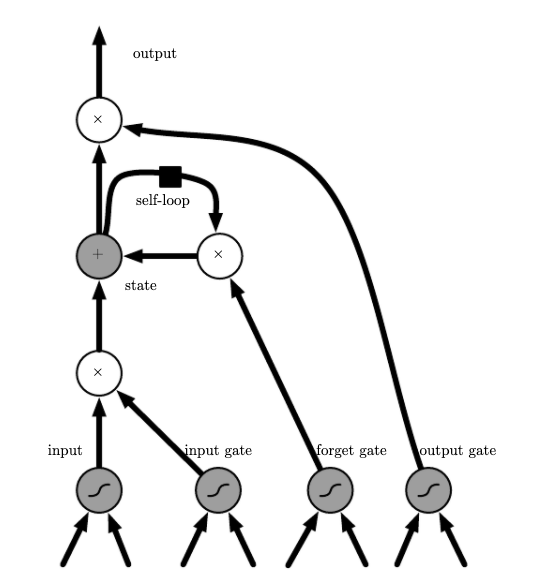
\includegraphics[scale=0.3]{LSTM}
            \end{center}

            Instead of a unit that simply applies an element-wise nonlinearity to the affine transformation of inputs and
            recurrent units, LSTM recurrent networks have "LSTM" cells that have an internal recurrence, in addition to
            the outer recurrence of the RNN. Each cell has the same inputs and outputs as an ordinary recurrent network,
            but also has more parameters and a system of gating units that controls the flow of information. The most
            important component is the cell state unit, which has a linear self-loop. Here the self-loop weight is
            controlled by a forget gate unit. The learning equations for the LSTM cell are as follows:

            \begin{itemize}
                \item Input gate: $i_t = \sigma(W^{(ii)} \overline{x}_t + W^{(hi)} h_{t-1})$
                \item Forget gate: $f_t = \sigma(W^{(if)} \overline{x}_t + W^{(hf)} h_{t-1})$
                \item Output gate: $o_t = \sigma(W^{(io)} \overline{x}_t + W^{(ho)} h_{t-1})$
                \item Process input: $\overline{c}_t = tanh(W^{(i\overline{c})} + W^{(h\overline{c})} h_{t-1})$
                \item Cell update: $c_t = f_t * c_{t-1} + i_t + \overline{c}_t$
                \item Output: $y_t = h_t = o_t * tanh(c_t)$
            \end{itemize}

        \subsubsection{Gated Recurrent Units} \label{sec:GRU}
            Not all pieces of the LSTM architecture are actually necessary. The main difference with the LSTM and the
            GRU is that a single gating unity simultaneously controls the forgetting factor and the decision to update
            the state unit. The update equations are the following:

            \begin{itemize}
                \item Reset gate: $r_t = \sigma(W^{(ir)} \overline{x}_t + W^{(hr)}h_{t-1})$
                \item Update gate: $z_t = \sigma(W^{(iz)} \overline{x}_t + W^{(hz)}h_{t-1})$
                \item Process input: $\overline{h}_t = tanh(W^{(i\overline{h})} \overline{x}_t + r_t * (W^{(h\overline{h})}h_{t-1}))$
                \item Hidden state update: $h_t = (1-z_t)*h_{t-1} + z_t * \overline{h}_t$
                \item Output: $y_t = h_t$
            \end{itemize}

            The reset and update gates can individually "ignore" parts of the state vector. The update gates act like
            conditional leaky integrators that can linearly gate any dimension, thus choosing to copy it or completely
            ignore it by replacing it with the new target state value. The reset gates control which parts of the state
            get used to compute the next target state, introducing an additional nonlinear effect in the relationship
            between past state and future state.
    
    \subsection{Attention} \label{sec:Attention}
        Attention is a mechanism for alignment in models where the output and input are of variable-length. This lets us
        align inputs with their corresponding outputs in applications such as machine translation, image captioning and
        more. Attention in machine translation is where we align each output word with relevant input words by computing
        a \hyperref[sec:Softmax]{softmax} of the inputs as follows.
        
        Context vector $c_i$: weighted sum of input encodings $h_j$
        $$ c_i = \sum_j a_{ij}h_j $$

        $a_{ij}$ is an alignment weight between input encoding $h_j$ and output encoding $s_i$.
        $$ a_{ij} = \frac{exp(alignment(s_i, h_j))}{\sum_{ji} exp(alignment(s_i, h_{j'}))} $$

        Alignment example: $alignment(s_i, h_j) = s^T_i h_j$

    \subsection{Training}
        To train a RNN, the trick is to unroll it through time and then use regular \hyperref[sec:Backprop]{back
        propagation}. This strategy is called backpropagation through time. The algorithm will also consider weight sharing will also play a part where
        we combine gradients of shared weights into a single gradient. 
        
        There is first a forward pass through the unrolled network. Then the output sequence is evaluated using a cost
        function. The gradients of that cost function are then propagated backward through the unrolled network. Finally
        the model parameters are updated using the gradients computed during backpropagation through time. 

        \subsubsection{Challenges}
            Some challenges that training brings up, is the \hyperref[sec:VanishingProblem]{gradient vanishing and
            explosion} problem. Another issue is the Long Range memory problem, although a RNN can handle sequences of events
            but there is no guarantee it will remember information from the first input. This is specifically important
            applications like machine translation where every input is equally important so you need the long term memory.
            Lastly, prediction drift is another challenge when training RNN's. Prediction drift is the idea that predictions
            far into the future will have error from the previous predictions propagated through to it and therefore be
            less accurate.


\printindex

\end{document}
